% QUANTUM CHANNELS
\section*{Representations of quantum channels}
\noindent A state of a quantum system with $D$ different configurations can be described by a \textit{density matrix} $\rho \in \mathbb{C}^{D \times D}$ with $\rho \geq 0$ and $\tr[\rho] = 1$. A linear map $\mathcal{E}: \mathbb{C}^{D \times D} \rightarrow \mathbb{C}^{D \times D}$ is called
\begin{itemize}
	\item \textit{positive} if $\mathcal{E}(X) \geq 0$ for all $X \geq 0$,
	\item \textit{completely positive} (CP) if $\mathcal{E} \otimes \mathrm{id}_n$ is positive for all $n \in \mathbb{N}$, where $\mathrm{id}_n$ is the identity map on $\mathbb{C}^{n \times n}$ such that $\mathcal{E} \otimes \mathrm{id}_n: X \otimes Y \mapsto \mathcal{E}(X) \otimes Y$,
	\item \textit{trace preserving} (TP) if $\tr[\mathcal{E}(X)] = \tr[X]$ for all $X$,
	\item \textit{unital} (U) if $\mathcal{E}(\mathbbm{1}) = \mathbbm{1}$.
\end{itemize}
A CPTP map is called a \textit{quantum channel}, mapping density matrices to density matrices. It has the following representations:
\begin{itemize}
	\item \textit{Choi-Jamiolkowski isomorphism}: For the maximally entangled state $\tket{\Omega} = \sum\limits_{\alpha = 1}^D \tket{\alpha, \alpha} \in \mathbb{C}^D \otimes \mathbb{C}^D$, the Choi matrix
	\begin{equation}
		C_{\mathcal{E}} = (\mathcal{E} \otimes \mathrm{id}) (\tket{\Omega} \tbra{\Omega}) \overset{\mathrm{CP}}{\geq} 0 \: \text{ with } \tr_1[C_{\mathcal{E}}] \overset{\mathrm{TP}}{=} \mathbbm{1}
	\end{equation}
	defines a bijection $\mathcal{E} \mapsto C_{\mathcal{E}}$.
	
	\item \textit{Kraus representation}: There exist Kraus operators $\{A^s \in \mathbb{C}^{D \times D}\}_{s=1}^d$ such that
	\begin{equation}
		\mathcal{E}(X) \overset{\mathrm{CP}}{=} \sum_{s=1}^d A^s X {A^s}^{\dagger} \: \text{ with }  \sum_{s=1}^d {A^s}^{\dagger} A^s \overset{\mathrm{TP}}{=} \mathbbm{1}.
	\end{equation}
	
	\item \textit{Transfer matrix}: Using the isomorphism $\tket{\alpha}\tbra{\beta} \leftrightarrow \tket{\alpha, \beta} $ between $\mathbb{C}^{D \times D}$ and $\mathbb{C}^{D^2}$, with the relation
	\begin{equation}
		( \gamma \vert \mathcal{E}( \tket{\alpha} \tbra{\beta} ) \vert \delta ) = \tbra{\gamma, \delta} T_{\mathcal{E}} \tket{\alpha, \beta},
	\end{equation}
	we get the matrix representation
	\begin{equation}
		T_{\mathcal{E}} \overset{\mathrm{CP}}{=} \sum_{s=1}^d A^s \otimes \overline{A^s} \: \text{ with }  \tbra{\mathbbm{1}} T_{\mathcal{E}} \overset{\mathrm{TP}}{=} \tbra{\mathbbm{1}}.
	\end{equation}
\end{itemize}

\noindent A linear map $\mathcal{E}$ is CPTP if and only if the corresponding \textit{dual map} $\mathcal{E}^*$, defined via $\mathrm{tr}[\mathcal{E}(X) Y] = \mathrm{tr}[X \mathcal{E}^*(Y)]$ for all $X, Y \in \mathbb{C}^{D \times D}$, is CPU. It has Kraus representation $\mathcal{E}^*(X) = \sum_{s} {A^s}^{\dagger} X A^s$ and transfer matrix $T_{\mathcal{E}^*} = T_{\mathcal{E}}^{\dagger}$. \cite{wolf2012channels, wolf2022information} \\

\noindent The Kraus operators $\{A^s \in \mathbb{C}^{D \times D}\}_{s=1}^d$ can equivalently be seen as a rank-3 tensor $A \in \mathbb{C}^{d \times D \times D}$, which links quantum channels to uniform MPS. Making analytical proofs more convenient, we define the latter with periodic boundary conditions here. Namely, for $d$-dimensional spins on a chain of length $N$ \cite{cirac2021matrix}:
\begin{equation}
	\ket{\psi(A,N)} = \sum_{s_1, \ldots, s_N = 1}^d \tr[A^{s_1} \cdots A^{s_N}]\ket{s_1 \ldots s_N} \in \mathbb{C}^{d^N}.
\end{equation}


% PRIMITIVITY
\section*{Primitivity} 
\noindent As for every linear map with equal input and output space, we can assign a \textit{spectrum} to a quantum channel:
\begin{align}
\begin{split}
	\sigma(\mathcal{E}) &= \{\lambda \in \mathbb{C} \mid \mathcal{E}(X) = \lambda X \text{ for some nonzero } X \in \mathbb{C}^{D \times D} \} \\
	&= \{\lambda \in \mathbb{C} \mid  T_{\mathcal{E}}\tket{X} = \lambda \tket{X} \text{ for some nonzero } \tket{X} \in \mathbb{C}^{D^2} \}.
\end{split}
\end{align}
It is easy to show that the dual map $\mathcal{E}^*$ has the same spectrum, with equal multiplicities for every eigenvalue. The \textit{spectral radius} $\rho$ is defined as the maximum magnitude in the spectrum, equal to 1 for TP maps:
\begin{equation}
	\rho(\mathcal{E}) = \max\{\vert \lambda \vert \mid \lambda \in \sigma(\mathcal{E})\} \overset{\mathrm{TP}}{=} 1.
\end{equation}
An important part of the spectrum in the context of MPS is the \textit{peripheral spectrum}, consisting of all eigenvalues with absolute value equal to the spectral radius:
\begin{equation}
	\sigma_p(\mathcal{E}) = \{\lambda \in \sigma(\mathcal{E}) \mid \vert\lambda\vert = 1\}.
\end{equation}
It turns out that for quantum channels the peripheral spectrum has trivial Jordan blocks, i.e. equal algebraic and geometric multiplicities. This is very useful for the following two spectral properties \cite{wolf2012channels}:
\begin{itemize}
	\item \textit{Irreducibility}: The spectral radius one is a nondegenerate eigenvalue with positive definite right eigenvector $r > 0$ (and left eigenvector $\mathbbm{1}$). The other eigenvalues of magnitude one turn out to be the other $p$-th roots of one for some $p \leq D^2$, so that $T_{\mathcal{E}}$ can be written as
	\begin{equation}
	T_{\mathcal{E}} = \tket{r}\tbra{\mathbbm{1}} + \sum\limits_{j=1}^{p-1}e^{i2\pi j/p} \tket{r_j}\tbra{l_j} + \mathcal{O}(\vert \lambda_2 \vert) \:\:\mathrm{with}\:\: \vert \lambda_2 \vert < 1.
	\end{equation}
	The eigenvectors fulfill the orthonormality conditions 
	\begin{equation}
	( \mathbbm{1} \vert r ) = \tr [r] = 1, \:\: ( \mathbbm{1} \vert r_j ) = \tr [r_j] = 0, \:\: ( l_j \vert r_k ) = \tr [l_j^{T} r_k] = \delta_{jk}.
	\end{equation}
	
	\item \textit{Primitivity}: $\mathcal{E}$ is irreducible and has trivial peripheral spectrum, i.e. counting algebraic multiplicities, there is only one eigenvalue of magnitude and value one and the corresponding eigenvector $r$ is positive definite:
	\begin{equation}
		T_{\mathcal{E}} = \tket{r}\tbra{\mathbbm{1}} + \mathcal{O}(\vert \lambda_2 \vert) \:\:\mathrm{with}\:\: \vert \lambda_2 \vert < 1.
	\end{equation}
\end{itemize}

\noindent In the main text, we defined primitivity for a general, completely positive map with dominant eigenvectors $r, l$. Here, we always work with the special cases of CPTP or CPU maps. However, this is not a restriction. Trace preservation (left isometric gauge) can be achieved with the similarity transformation $A^s \rightarrow \overline{l}^{1/2} A^s \overline{l}^{-1/2}$, unitality (right isometric gauge) with $A^s \rightarrow r^{-1/2} A^s r^{1/2}$. Both are gauge transformations of the form $A^s \rightarrow S A^s S^{-1}$, leaving the uMPS invariant for any invertible $S \in \mathbb{C}^{D \times D}$. \\

\noindent To get a physical intuition for irreducibility and primitivity, we want to make two examples for $d = 2$ \cite{perez2007matrix}: 
\begin{itemize}
	\item Antiferromagnetic GHZ state $\ket{\psi(A)} = \ket{0101 \ldots} + \ket{1010 \ldots}$ with 
	\begin{equation}
		A^0 = \begin{pmatrix} 0 & 1 \\ 0 & 0 \end{pmatrix} \in \mathbb{C}^{2 \times 2}, \: A^1 = \begin{pmatrix} 0 & 0 \\ 1 & 0 \end{pmatrix} \in \mathbb{C}^{2 \times 2}.
	\end{equation}
	The corresponding quantum channel $\mathcal{E}_A: \mathbb{C}^{2 \times 2} \rightarrow \mathbb{C}^{2 \times 2}$, $X \mapsto \sum_s A^s X {A^s}^{\dagger}$ is irreducible with $p = 2$, since $\mathcal{E}_A^*(\mathbbm{1}) = \mathbbm{1}$ and $\mathcal{E}_A^*(\sigma^z) = -\sigma^z$ are the only peripheral left eigenvector equations.
	\item Ferromagnetic product state $\ket{\psi(A)} = \ket{0000 \ldots}$ with $A^0 = (1) \in \mathbb{C}^{1 \times 1}$, $A^1 = (0) \in \mathbb{C}^{1 \times 1}$. The corresponding quantum channel $\mathcal{E}_A: \mathbb{C} \rightarrow \mathbb{C}$, $x \mapsto A^0 x {A^0}^{\dagger} = x$ is primitive. 
	\end{itemize}

% primitivity, injectivity, invertibility
\noindent In the literature, the terms \textit{primitivity}, \textit{injectivity} and \textit{invertibility} are interchangeably used. Let us order them with the following theorem \cite{fernandez2015frustration}:
\begin{theorem}{Primitivity, injectivity, invertibility}{primitivity_injectivity_invertibility}
For a CPTP map $\mathcal{E}_A$, represented by the rank-3 tensor $A \in \mathbb{C}^{d \times D \times D}$, the following are equivalent:
\begin{enumerate}
	\item[(1)] $\mathcal{E}_A$ is \textit{primitive}.
	\item[(2)] There exists a finite $L_0 \in \mathbb{N}$ such that for all $L \geq L_0$: 
	\begin{equation}
		\mathrm{span}\{A^{s_1} \cdots A^{s_L}\}_{s_1, \ldots, s_L} = \mathbb{C}^{D \times D}.
	\end{equation}
	\item[(3)] For all $L \geq L_0$, the map $\Gamma_{A^L}: \mathbb{C}^{D \times D} \rightarrow \mathbb{C}^{d^{L}}$, defined by 
	\begin{equation}
		\Gamma_{A^L}(X) = \sum\limits_{s_1, \ldots, s_L}\mathrm{tr}[X A^{s_1} \cdots A^{s_L}]\ket{s_1 \ldots s_L},
	\end{equation}
	is \textit{injective}.
	\item[(4)] For all $L \geq L_0$, the blocked tensor $A^L$ is \textit{invertible} with respect to the physical leg, i.e. there exists a tensor $A^{-1} \in \mathbb{C}^{d^L \times D \times D}$ such that 
	\begin{equation}
		\sum\limits_{s_1, \ldots, s_L} (A^{s_1} \cdots A^{s_L})_{\alpha, \beta}(A^{-1})^{s_1, \ldots, s_L}_{\gamma, \delta} = \delta_{\alpha \gamma} \delta_{\beta \delta}.
	\end{equation}
\end{enumerate}
If $\Gamma_{A^L}$ is injective, $\Gamma_{B A^L}$ and $\Gamma_{A^L C}$ are injective for any nonzero tensors $B, C$.
\end{theorem}
% proof
\begin{proof}
$(1) \Leftrightarrow (2)$: Theorem \ref{thm:primitive_cptp} below. \\

\noindent In the following we summarize the indices $(s_1, \ldots, s_L)$ in the multi-index $S \in \{0, \ldots, d^{L} - 1\}$. \\

\noindent $(2) \Leftrightarrow (3)$:  $\mathrm{span}\{A^S\}= \mathbb{C}^{D \times D}$ $\Leftrightarrow$ for every nonzero $X \in \mathbb{C}^{D \times D}$ there is $S$ such that $\tr[XA^S] \neq 0$ $\Leftrightarrow$ $\tr[XA^S] = 0$ for all $S$ implies $X=0$ $\Leftrightarrow$ $\Gamma_{A^L}(X)=0$ implies $X=0$ $\Leftrightarrow$ $\Gamma_{A^L}$ is injective. \\

\noindent $(2) \Rightarrow (4)$:  Let $\tket{a_{\gamma\delta}} \in \mathbb{C}^{d^L}$ be the coefficient vector corresponding to $\tket{\gamma}\tbra{\delta}$, i.e. $\tket{\gamma}\tbra{\delta} = \sum_S ( S  \vert a_{\gamma\delta} ) A^S$.
Define $(A^{-1})^S_{\gamma\delta} := ( S \vert a_{\gamma\delta} )$ and it follows 
\begin{equation}
	\sum_S A^S_{\alpha\beta} (A^{-1})^S_{\gamma\delta} = \tbra{\alpha} \left[ \sum_S ( S \vert a_{\gamma\delta} ) A^S \right] \tket{\beta} = ( \alpha \vert \gamma ) ( \delta \vert \beta ) = \delta_{\alpha \gamma} \delta_{\beta \delta}.
\end{equation}
\noindent $(4) \Rightarrow (2)$: For any $X \in \mathbb{C}^{D \times D}$ define $( S \vert a_X ) := \tr[X^T (A^{-1})^S]$. Then 
\begin{align}
\begin{split}
	\sum_S ( S \vert a_{X} ) A^S &= \sum_{\alpha,\beta}\sum_{\gamma,\delta} \tbra{\delta} X^T \tket{\gamma} \left[ \sum_S \tbra{\alpha}A^S \tket{\beta}\tbra{\gamma} (A^{-1})^S \tket{\delta} \right] \tket{\alpha} \tbra{\beta} \\
	&= \sum_{\alpha,\beta} \tbra{\beta} X^T \tket{\alpha}\tket{\alpha}\tbra{\beta} = X. 
\end{split}
\end{align}

\noindent Assume that $\Gamma_{A^L}$ is injective and the tensor $B \in \mathbb{C}^{d_B \times D \times D}$ nonzero. The $\Gamma$-function of the product tensor $B A^L$ is given by
\begin{equation}
	\Gamma_{B A^L}(X) = \sum_{s, S} \tr[X B^s A^S]\ket{s, S} = \sum_s \ket{s} \otimes \Gamma_{A^L}(X B^s).
\end{equation}
It holds: $\Gamma_{B A^L}(X) = 0$ $\Leftrightarrow$ $\Gamma_{A^L}(X B^s) = 0$ for all $s$ $\Leftrightarrow$ $X B^s = 0$ for all $s$ $\Leftrightarrow$ $X=0$, where we used injectivity of $\Gamma_{A^L}$ for the second equivalence. Consequently $\Gamma_{B A^L}$ is also injective. The proof for $\Gamma_{A^L C}$ with nonzero $C \in \mathbb{C}^{d_C \times D \times D}$ works the same way.
\end{proof}

% primitive CPTP maps
\noindent We still owe the proof for $(1) \Leftrightarrow (2)$, which we provide with an extra theorem \cite{wolf2012channels}:
\begin{theorem}{Primitive CPTP maps}{primitive_cptp}
Let $\mathcal{E}: \mathbb{C}^{D \times D} \rightarrow \mathbb{C}^{D \times D}$ be a completely positive trace preserving map with Kraus representation $\mathcal{E}(X) = \sum_{s=1}^d A^s X {A^s}^{\dagger}$ and Choi matrix $C_{\mathcal{E}} = (\mathcal{E} \otimes \mathrm{id})(\ket{\Omega}\bra{\Omega})$ such that $d \geq \mathrm{rank}(C_{\mathcal{E}})$. The following properties are equivalent:
\begin{enumerate}
	\item[(1)] Primitivity: There exists a positive definite $r \in \mathbb{C}^{D \times D}$ with unit trace such that
	\begin{equation}
		T_{\mathcal{E}} = \tket{r}\tbra{\mathbbm{1}} + \mathcal{O}(\vert \lambda_2 \vert) \:\:\mathrm{with}\:\: \vert \lambda_2 \vert < 1.
	\end{equation}
	
	\item[(2)] Eventual strict positivity: There exists a minimal $M_0 \in \mathbb{N}$ such that for all $M \geq M_0$ and nonzero positive semidefinite $X \in \mathbb{C}^{D \times D}$: 
	\begin{equation}
		\mathcal{E}^M(X) > 0.
	\end{equation}
	
	\item[(3)] Eventual full Kraus rank: There exists a minimal $L_0 \in \mathbb{N}$ such that for all $L \geq L_0$: 
	\begin{equation}
		\mathrm{rank}(C_{\mathcal{E}^L}) = D^2.
	\end{equation}
	\item[(4)] There exists a minimal $L_0 \in \mathbb{N}$ such that for all $L \geq L_0$: 
	\begin{equation}
		\mathrm{span}\{A^{s_1}\cdots A^{s_L}\} = \mathbb{C}^{D \times D}.
	\end{equation}
\end{enumerate}
The $L_0$s in (3) and (4) are the same. Moreover, $M_0 \leq L_0$.
\end{theorem}
% proof
\begin{proof}
We prove $(1) \Rightarrow (3) \Rightarrow (2) \Rightarrow (1)$ and $(3) \Leftrightarrow (4)$. \\

\noindent $(1) \Rightarrow (3)$: Primitivity implies $\lim_{L \to \infty} \mathcal{E}^L(X) \eqqcolon \mathcal{E}^{\infty}(X) = r \tr[X]$ and thus the following convergence for the Choi matrix:
\begin{equation}
	\lim_{L \to \infty} C_{\mathcal{E}^L} = (\mathcal{E}^{\infty} \otimes \mathrm{id})(\tket{\Omega} \tbra{\Omega}) = r \otimes \mathbbm{1},
\end{equation}
with $r > 0$. If $C_{\mathcal{E}^L}$ had a kernel for all $L$, with eigenvector $\tket{\psi_L}$, we could derive the following bound for the minimal eigenvalue of $r$:
\begin{align}
\begin{split}
	\lambda_{\mathrm{min}}(r) &\leq \vert \tbra{\overline{\psi_L}} C_{\mathcal{E}^L} - r \otimes \mathbbm{1} \tket{\psi_L} \vert \leq \Vert C_{\mathcal{E}^L} - r \otimes \mathbbm{1} \Vert = \Vert [(\mathcal{E}^L - \mathcal{E}^{\infty}) \otimes \mathrm{id}] [\tket{\Omega} \tbra{\Omega} - r \otimes \mathbbm{1}] \Vert \\
	& \leq \mu^L c \Vert \tket{\Omega} \tbra{\Omega} - r \otimes \mathbbm{1} \Vert,
\end{split}
\end{align}
where $\Vert \cdot \Vert$ is the operator norm, $\vert \lambda_2 \vert < \mu < 1$ and $c > 0$. So for sufficiently large $L$ the bound contradicted $r > 0$. As a consequence, there has to be a finite $L_0 \in \mathbb{N}$ such that for all $L \geq L_0$: $C_{\mathcal{E}^L} > 0$, implying $\mathrm{rank}(C_{\mathcal{E}^L}) = D^2$. \\

\noindent $(3) \Rightarrow (2)$: For $\tket{\psi}, \tket{\varphi} \in \mathbb{C}^D$ and $X \in \mathbb{C}^{D \times D}$ the following implications hold:
\begin{align}
\begin{split}
C_{\mathcal{E}^{L_0}}>0 &\:\:\Rightarrow\:\: \tbra{\overline{\varphi}, \psi} C_{\mathcal{E}^{L_0}} \tket{\varphi,\overline{\psi}} > 0 \:\:\text{for all nonzero}\: \tket{\psi}, \tket{\varphi} \\
&\:\:\Rightarrow\:\: \tbra{\overline{\varphi}} \mathcal{E}^{L_0} \left( \tket{\psi}\tbra{\overline{\psi}} \right) \tket{\varphi} > 0 \:\:\text{for all nonzero}\: \tket{\psi},\tket{\varphi} \\
&\:\:\Rightarrow\:\: \mathcal{E}^{L_0} \left( \tket{\psi}\tbra{\overline{\psi}} \right) > 0 \:\:\text{for all nonzero}\: \tket{\psi} \\
&\:\:\Rightarrow\:\: \mathcal{E}^{L_0}(X) > 0 \:\:\text{for all nonzero}\: X\geq0.
\end{split}
\end{align}
From the first to the second line we used 
\begin{align}
\begin{split}
\tbra{\overline{\varphi},\psi} C_{\mathcal{E}^{L_0}} \tket{\varphi,\overline{\psi}} 
&= \tbra{\overline{\varphi},\psi} (\mathcal{E}^{L_0}\otimes\mathrm{id})(\tket{\Omega}\tbra{\Omega}) \tket{\varphi,\overline{\psi}} 
= \sum_{\alpha,\beta} \tbra{\overline{\varphi}} \mathcal{E}^{L_0}(\tket{\alpha}\tbra{\beta})\tket{\varphi} ( \psi \vert \alpha ) ( \beta \vert \overline{\psi} ) \\
&= \tbra{\overline{\varphi}} \mathcal{E}^{L_0} \left( \tket{\psi}\tbra{\overline{\psi}} \right) \tket{\varphi}.
\end{split}
\end{align}
This also shows that $M_0 \leq L_0$. For $M \geq M_0$, $\mathcal{E}^{M-M_0}(X)$ is nonzero and positive semidefinite if $X$ is so, since $\mathcal{E}$ is trace preserving and positive. As a consequence $\mathcal{E}^{M}(X) = \mathcal{E}^{M_0}(\mathcal{E}^{M-M_0}(X)) > 0$ if $\mathcal{E}^{M_0}(X) > 0$. \\

\noindent $(2) \Rightarrow (1)$: We show that if $\mathcal{E}$ is not primitive, there is a nonzero $X \geq 0$ such that $\mathcal{E}^n(X)$ is not full rank for all $n \in \mathbb{N}$. Denote by $r$ a positive semidefinite fixed point, which always exists for a positive TP map. Then primitivity can be violated in the following three ways:
\begin{enumerate}
	\item[(i)] $r$ is not full rank \:$\Rightarrow$\: $\mathcal{E}^n(r) = r$ is not full rank for all $n \in \mathbb{N}$.
	\item[(ii)] There is another eigenvector $\Tilde{r}$ corresponding to the eigenvalue 1, which can be taken Hermitian since $\mathcal{E}$ is positive \:$\Rightarrow$\: $\lambda_{\mathrm{max}} r - \Tilde{r}$ with $\lambda_{\mathrm{max}} := \max \sigma(r^{-1/2}\Tilde{r}r^{-1/2})$ is a positive semidefinite fixed point that does not have not full rank $\Rightarrow$ (i) for $\lambda_{\mathrm{max}} r - \Tilde{r}$.
	\item[(iii)] There is another eigenvalue $\Tilde{\lambda}$ with modulus 1, which has to be another $p$-th root of unity for some $p \leq D^2$ \:$\Rightarrow$\: (ii) for $\mathcal{E}^p$. 
\end{enumerate}

\noindent$(3) \Leftrightarrow (4)$: For $\tket{\psi} \in\mathbb{C}^D\otimes\mathbb{C}^D$, $X \in \mathbb{C}^{D \times D}$ and the multi-index $S = (s_1, \ldots, s_{L_0})$ the following equivalences hold:
\begin{align}
\begin{split}
\mathrm{rank}(C_{\mathcal{E}^{L_0}}) = D^2 &\:\:\Leftrightarrow\:\: C_{\mathcal{E}^{L_0}} > 0 \:\:\Leftrightarrow\:\: \tbra{\overline{\psi}} C_{\mathcal{E}^{L_0}} \tket{\psi} > 0 \:\:\text{for all nonzero}\: \tket{\psi} \\
&\:\:\Leftrightarrow\:\: \sum\nolimits_S \vert \tbra{\overline{\psi}} A^S \otimes \mathbbm{1}\tket{\Omega} \vert^2 > 0 \:\:\text{for all nonzero}\: \tket{\psi} \\
&\:\:\Leftrightarrow\:\: \text{for every nonzero } \tket{\psi} \text{ there is } S \text{ such that } \tbra{\overline{\psi}} A^S \otimes \mathbbm{1}\tket{\Omega} \neq 0 \\
\mathrm{span}\{A^S\} = \mathbb{C}^{D \times D} &\:\:\Leftrightarrow\:\: \text{for every nonzero } X \text{ there is } S \text{ such that } \tr[X^{\dagger} A^S] \neq 0 \\
\end{split}
\end{align} 
For $C_{\mathcal{E}^{L_0}} > 0$ there is a constant $c > 0$ so that $C_{\mathcal{E}^{L_0}} \geq cC_{\mathcal{E}^{L_0-1}} \geq 0$. It follows for $L_0+1$ and by induction for all integers larger than $L_0$: $C_{\mathcal{E}^{L_0+1}} = (\mathcal{E} \otimes \mathbbm{1})(C_{\mathcal{E}^{L_0}}) \geq c (\mathcal{E} \otimes \mathbbm{1})(C_{\mathcal{E}^{L_0-1}}) = cC_{\mathcal{E}^{L_0}} > 0$.
\end{proof}


\noindent From theorem \ref{thm:primitivity_injectivity_invertibility} we can make the following important conclusion about the genericness of primitive tensors: For $d$ randomly drawn matrices $\{A^s\}_{s=1}^d$, the dimension of $\mathrm{span}\{A^{s_1} \cdots A^{s_L}\}$ is expected to grow as $d^L$ until it reaches $D^2$. Therefore, a generic rank-3 tensor is expected to be primitive with $L_0 \sim 2 \ln D / \ln d$, whereas non-primitive tensors appear with measure zero in the space $\mathbb{C}^{D \times d \times D}$. \cite{perez2007matrix} \\


% FUNDAMENTAL THEOREM
\newpage
\section*{Fundamental theorem}
In general, it can be proven that $\ket{\psi(A,N)} = \ket{\psi(B,N)}$ if and only if $B^s = S A^s S^{-1}$ with $S \in \mathbb{C}^{D \times D}$ invertible. Here, we prove this under the assumption of primitivity and unitality, which requires $S$ to be unitary \cite{cirac2017matrix}:

% fundamental theorem
\begin{theorem}{Fundamental theorem}{fundamental_theorem}
For tensors $A \in \mathbb{C}^{d \times D_A \times D_A}$ and $B \in \mathbb{C}^{d \times D_B \times D_B}$ with corresponding primitive CPU maps $\mathcal{E}_A$ and $\mathcal{E}_B$, the following are equivalent (for some phases $\alpha,\beta \in \mathbb{C}$):
\begin{enumerate}
	\item[(1)] $\ket{\psi(B,N)} = e^{i \alpha} \ket{\psi(A,N)}$,
	\item[(2)]  $D_A = D_B \eqqcolon D$ and there exists unitary $U \in \mathbb{C}^{D \times D}$ such that 
	\begin{itemize}
		\item $\mathcal{E}_{AB}(U) = e^{i\beta}U$ with 1 the spectral radius,
		\item $B^s = e^{-i\beta}U^{\dagger} A^s U$ for all $s$.
	\end{itemize}
\end{enumerate}
\end{theorem}
% proof
\begin{proof}
\noindent $(2) \Rightarrow (1)$: Trivial insertion of the MPS definition and use of the trace cyclicity:
\begin{align}
\begin{split}
	\ket{\psi(B,N)} &= \sum_{s_1,...,s_N} \tr[B^{s_1} \cdots B^{s_N}]\ket{s_1 \ldots s_N} \\
	&= e^{-i\beta N} \sum_{s_1, \ldots, s_N} \tr[U^{\dagger} A^{s_1} U \cdots U^{\dagger} A^{s_N} U]\ket{s_1 \ldots s_N} \\
	&= e^{-i\beta N}\sum_{s_1,...,s_N} \tr[A^{s_1} \cdot\cdot\cdot A^{s_N}]\ket{s_1 \ldots s_N} \\
	&= e^{-i \beta N} \ket{\psi(A,N)}.
\end{split}
\end{align}

\noindent $(1) \Rightarrow (2)$: $T_A = \sum_s A^s \otimes \overline{A^s}$ is the transfer matrix of $\mathcal{E}_A: X \mapsto \sum_s A^s X {A^s}^{\dagger}$ in the basis of matrix units. In the same manner we define the mixed transfer matrix $T_{AB} \coloneqq \sum_s A^s \otimes \overline{B^s}$ of $\mathcal{E}_{AB}: X \mapsto \sum_s A^s X {B^s}^{\dagger}$. We first show that $\ket{\psi(B,N)} = e^{i \alpha} \ket{\psi(A,N)}$ implies spectral radius 1 for $\mathcal{E}_{AB}$. Inserting the MPS definition and using trace properties we have
\begin{align}
\begin{split}
	\langle \psi(A,N) \vert \psi(A,N) \rangle &= \sum_{s_1, \ldots, s_N} \tr[A^{s_1} \cdots A^{s_N}] \overline{\tr[A^{s_1} \cdots A^{s_N}]} \\
	&= \sum_{s_1, \ldots, s_N} \tr\left[A^{s_1} \cdots A^{s_N} \otimes \overline{A^{s_1}} \cdots \overline{A^{s_N}}\:\right] \\
	&= \tr[T_A^N].
\end{split}
\end{align}
As $\mathcal{E}_A$ is CPU primitive, we can write $T_A = \tket{\mathbbm{1}} \tbra{l_A} + \mathcal{O}(\vert \lambda_2 \vert)$ with $\vert \lambda_2 \vert < 1$ the second largest eigenvalue magnitude. So $\langle \psi(A,N) \vert \psi(A,N) \rangle = \tr[T_A^N]$ equals  $( l_A \vert \mathbbm{1} ) = \tr[l_A] = 1$ up to a correction exponentially small in $N$. In the same manner we compute the mixed overlap
\begin{align}
\begin{split}
	\langle \psi(B,N) \vert \psi(A,N) \rangle &= \sum_{s_1, \ldots, s_N} \tr[A^{s_1} \cdots A^{s_N}]\overline{\tr[B^{s_1} \cdots B^{s_N}]} \\
	&= \sum_{s_1, \ldots, s_N} \tr\left[A^{s_1} \cdots A^{s_N} \otimes \overline{B^{s_1}} \cdots \overline{B^{s_N}}\:\right] \\
	&= \tr[T_{AB}^N].
\end{split}
\end{align}
Taken together, $\ket{\psi(B,N)} = e^{i \alpha} \ket{\psi(A,N)}$ and $\lim\limits_{N \to \infty} \langle \psi(A,N) \vert \psi(A,N) \rangle = 1$ imply 
\begin{equation}
	\lim\limits_{N \to \infty} \vert \langle \psi(B,N) \vert \psi(A,N) \rangle \vert = 1 = \lim\limits_{N \to \infty} \vert \tr[T_{AB}^N] \vert.
\end{equation}

\noindent So $\mathcal{E}_{AB}$ has spectral radius 1. Next we show that $\mathcal{E}_{AB}(X) = e^{i\beta}X$ for some $X$ implies $X =: U$ is unitary and $B^s = e^{-i\beta}U^{\dagger} A^s U$ for all $s$. For this consider the general eigenvalue equation for $X \in \mathbb{C}^{D_A \times D_B}$.
\begin{equation}\label{eq_eigenvalue_equation}
	\mathcal{E}_{AB}(X) = \sum_s A^s X {B^s}^{\dagger} = \lambda X.
\end{equation}
Denoting by $l_B = \sqrt{l_B}\sqrt{l_B}$ the positive definite left leading eigenvector of $T_B$, we derive the upper bound
\begin{align}
\begin{split}
	\vert \lambda \vert \vert \tr[X l_B X^{\dagger}] \vert &= \left\vert \sum_s \tr[(X {B^s}^{\dagger} \sqrt{l_B})(\sqrt{l_B} X^{\dagger} A^s)] \right\vert \\
	&\leq \left(\sum_k\tr[X {B^s}^{\dagger} \sqrt{l_B} \sqrt{l_B} B^s X^{\dagger}]\right)^{1/2}\left(\sum_k\tr[\sqrt{l_B} X^{\dagger} A^s {A^s}^{\dagger} X \sqrt{l_B}]\right)^{1/2} \\
	&= \vert \tr[X l_B X^{\dagger}] \vert,
\end{split}
\end{align}
where we inserted (\ref{eq_eigenvalue_equation}) for the first equality and used $\mathcal{E}_A(\mathbbm{1}) = \sum_s A^s {A^s}^{\dagger} = \mathbbm{1}$, $\mathcal{E}_B^*(l_B) = \sum_s {B^s}^{\dagger} l_B B^s = l_B$, $\tr[X l_B X^{\dagger}] > 0$ for the last equality. The inequality results from the following two applications of Cauchy-Schwarz:
\begin{align}
\begin{split}
	\left\vert \sum_s \tr[X^sY^s] \right\vert &\leq \sum_s \left\vert \tr[X^sY^s] \right\vert \overset{\mathrm{CS}}{\leq} \sum_s \tr[{X^s}^{\dagger}X^s]^{1/2}\tr[{Y^s}^{\dagger} Y^s]^{1/2} \\
	& \overset{\mathrm{CS}}{\leq} \left(\sum_s\tr[{X^s}^{\dagger} X^s]\right)^{1/2}\left(\sum_s\tr[{Y^s}^{\dagger}Y^s]\right)^{1/2}.
\end{split}
\end{align}
So $\vert \lambda \vert \leq 1$. For $\vert \lambda \vert = 1$, Cauchy-Schwarz is fulfilled with an equal sign, implying proportionality $\sqrt{l_B} B^s X^{\dagger} = \mu \sqrt{l_B} X^{\dagger} A^s$. Since $l_B$ is nonsingular, this is equivalent to
\begin{equation}\label{eq_relation_A_B}
	B^s X^{\dagger} = \mu X^{\dagger} A^s.
\end{equation}
From 
\begin{equation}
		\overline{\mu} X = \overline{\mu} \sum_s A^s {A^s}^{\dagger} X = \overset{(\ref{eq_relation_A_B})}{=} \sum_s A^s X {B^s}^{\dagger} \overset{(\ref{eq_eigenvalue_equation})}{=} \lambda X	
\end{equation}
we get $\lambda = \overline{\mu} =: e^{i\beta}$, and from
\begin{equation}
	\mathcal{E}_B(X^{\dagger} X) = \sum_s B^s X^{\dagger} X {B^s}^{\dagger} \overset{(\ref{eq_relation_A_B})}{=} \vert \mu \vert^2  X^{\dagger} \left(\sum_s A^s {A^s}^{\dagger} \right) X = X^{\dagger} X
\end{equation}
we get $X^{\dagger} X = \mathbbm{1}$ and $D_A \geq D_B$ (since $\mathcal{E}_B$ is CPU primitive). Moreover, 
\begin{equation}
	\mathcal{E}_A^* (X l_B X^{\dagger}) = \sum_s {A^s}^{\dagger} X l_B X^{\dagger} A^s \overset{(\ref{eq_relation_A_B})}{=} X \left( \sum_s {B^s}^{\dagger} l_B B^s \right) X^{\dagger} = X l_B X^{\dagger}.
\end{equation}
So $X l_B X^{\dagger}$ is a fixed point of $\mathcal{E}_A^*$ which is not full rank if $D_A > D_B$, contradicting primitivity of $\mathcal{E}_A^*$. Consequently, $D_A = D_B \eqqcolon D$ and $X \eqqcolon U$ is unitary.
\end{proof}


% PARENT HAMILTONIAN
\section*{Parent Hamiltonian}
\noindent In the final chapter of this appendix, we want to find a local Hamiltonian for which the uMPS $\ket{\psi(A, N)}$ is the exact unique ground state, if it is generated by an invertible tensor $A$. \\

\noindent For $d$-dimensional spins, let $h = h^{\dagger} \in \mathbb{C}^{d^L \times d^L}$ be an interaction with interaction length $L$. The corresponding translational invariant Hamiltonian on $N$ sites is defined as 
\begin{equation}
	H = \sum_{n=1}^N h_n \:\:\mathrm{with}\:\: h_n = \mathbbm{1}_{\{1, \ldots, n-1\}} \otimes h_{\{n, \ldots, n+L-1\}} \otimes \mathbbm{1}_{\{n+L, \ldots, N\}}, \: N+1 \equiv  1.
\end{equation}
We call $h \geq 0$ \textit{parent interaction} if there is a rank-3 tensor $A \in \mathbb{C}^{d \times D \times D}$ such that 
\begin{equation}
	\mathrm{ker}(h) = \mathcal{G}_{A^L} = \mathrm{ran}(\Gamma_{A^L}) = \left\{ \sum\limits_{s_1, \ldots, s_L}\mathrm{tr}[X A^{s_1} \cdots A^{s_L}]\ket{s_1 \ldots s_L} \middle\vert X \in \mathbb{C}^{D \times D} \right\}.
\end{equation}
The corresponding Hamiltonian $H$ is called \textit{parent Hamiltonian}. Since the dimension of $\mathcal{G}_{A^L}$ is at most $D^2$, the parent Hamiltonian will necessarily be nontrivial as soon as $d^L > D^2$. \cite{cirac2021matrix}

% frustration freeness
\begin{theorem}{Frustration freeness}{frustration_free}
The parent Hamiltonian is \textit{frustration free}, in the sense that its ground space minimizes the energy locally:
\begin{equation} \label{eq_parent_hamiltonian}
	\mathrm{ker}(H) = \bigcap_{n=1}^N \mathrm{ker}(h_n).
\end{equation}
\end{theorem}
%proof
\begin{proof}
The Hamiltonian reads $H = \sum_{n=1}^N h_n$ with $h_n \geq 0$, $\mathrm{ker}(h_n) = \mathbb{C}^{d^{n-1}} \otimes \mathcal{G}_{A^L} \otimes \mathbb{C}^{d^{N-L-n+1}}$.
It is easy to check that $\ket{\psi(A,N)} \in \mathrm{ker}(h_n)$ for all $n$:
\begin{equation*}
	\ket{\psi(A,N)} = \sum_{s_1, \ldots, s_{n-1}} \sum_{s_{n+L}, \ldots, s_N} \ket{s_1 \ldots s_{n-1}} \otimes \underbrace{\Gamma_{A^L}\left(A^{s_{n+L}} \cdots A^{s_N} A^{s_1} \cdots A^{s_{n-1}} \right)}_{\in \mathcal{G}_{A^L}} \otimes \ket{s_{n+L} \ldots  s_N}.
\end{equation*}
This trivially implies $H\ket{\psi(A,N)} = 0$. Since $\bra{\varphi}H\ket{\varphi} = \sum_n  \bra{\varphi}h_n\ket{\varphi} \geq 0$ for all $\ket{\varphi} \in \mathbb{C}^{d^N}$, $\ket{\psi(A,N)}$ is a ground state of $H$. The whole ground space is given by $\mathrm{ker}(H)$ and the following inclusions hold:
\begin{equation}\label{eq_supset_kerH}
	\mathrm{ker}(H) \supseteq \bigcap_{n=1}^N \mathrm{ker}(h_n) \supseteq \left\{ \alpha\ket{\psi(A,N)} \mid \alpha \in \mathbb{C} \right\}. 
\end{equation}
To show inclusion in the other direction, first note that for $H \geq 0$, $H\ket{\varphi} = 0$ iff $\bra{\varphi}H\ket{\varphi} = 0$ \cite{tasaki2020physics}:
\begin{equation}
	H\ket{\varphi} = 0 \:\:\Leftrightarrow\:\: \sqrt{H}\ket{\varphi} = 0 \:\:\Leftrightarrow\:\: \Vert \sqrt{H}\varphi \Vert = 0 \:\:\Leftrightarrow\:\: \langle \sqrt{H}\varphi, \sqrt{H}\varphi \rangle = \bra{\varphi}H\ket{\varphi} = 0.
\end{equation}
Now, with $\bra{\varphi}h_n\ket{\varphi} \geq 0$ for all $n$, $\bra{\varphi}H\ket{\varphi} = \sum_n  \bra{\varphi}h_n\ket{\varphi} = 0$ implies $\bra{\varphi}h_n\ket{\varphi} = 0$ and thus $h_n\ket{\varphi} = 0$ for all $n$. So
\begin{equation}\label{eq_subset_kerH}
	\mathrm{ker}(H) \subseteq \bigcap_{n=1}^N \mathrm{ker}(h_n).
\end{equation}
\end{proof}

% intersection property
\begin{theorem}{Intersection property}{intersection_property}
Let $B \in \mathbb{C}^{d_B \times D \times D}$ be invertible, $A \in \mathbb{C}^{d_A \times D \times D}$, $C \in \mathbb{C}^{d_C \times D \times D}$. Then
\begin{equation}
	(\mathcal{G}_{A B} \otimes \mathbb{C}^{d_C}) \cap (\mathbb{C}^{d_A} \otimes \mathcal{G}_{B C}) = \mathcal{G}_{A B C}.
\end{equation}
\begin{equation*}
	\left\{ \raisebox{-0.5\height}{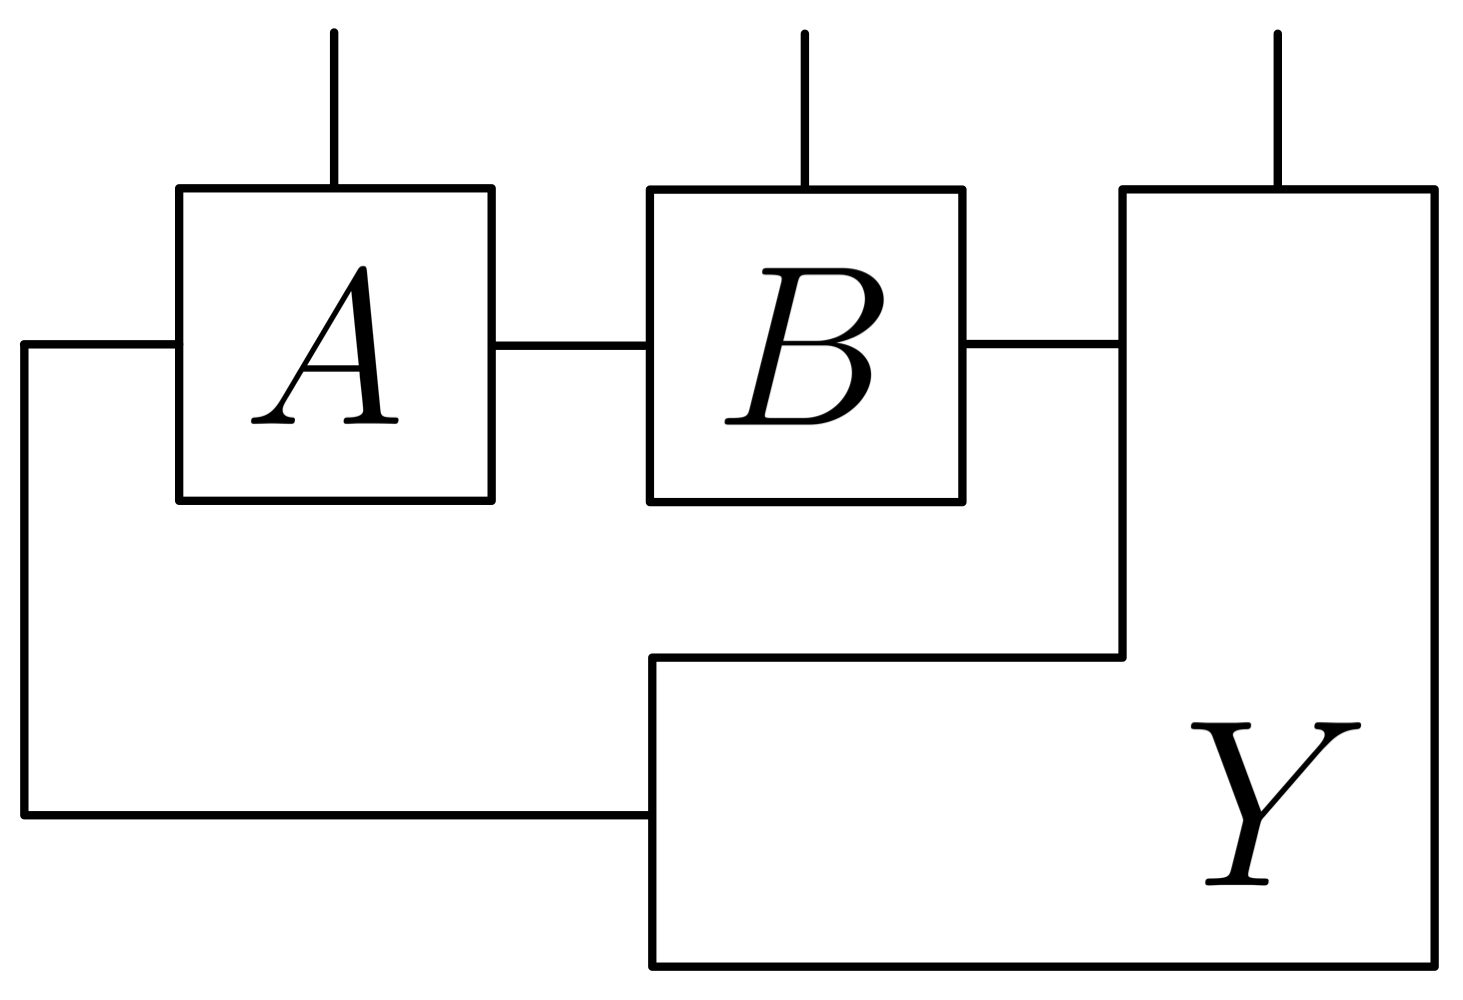
\includegraphics[height=2.2cm]{A_B_Y.png}} \: \middle\vert \: Y \in \mathbb{C}^{d_C \times D \times D} \right\} \:\:
	\cap 
	\:\: \left\{ \raisebox{-0.5\height}{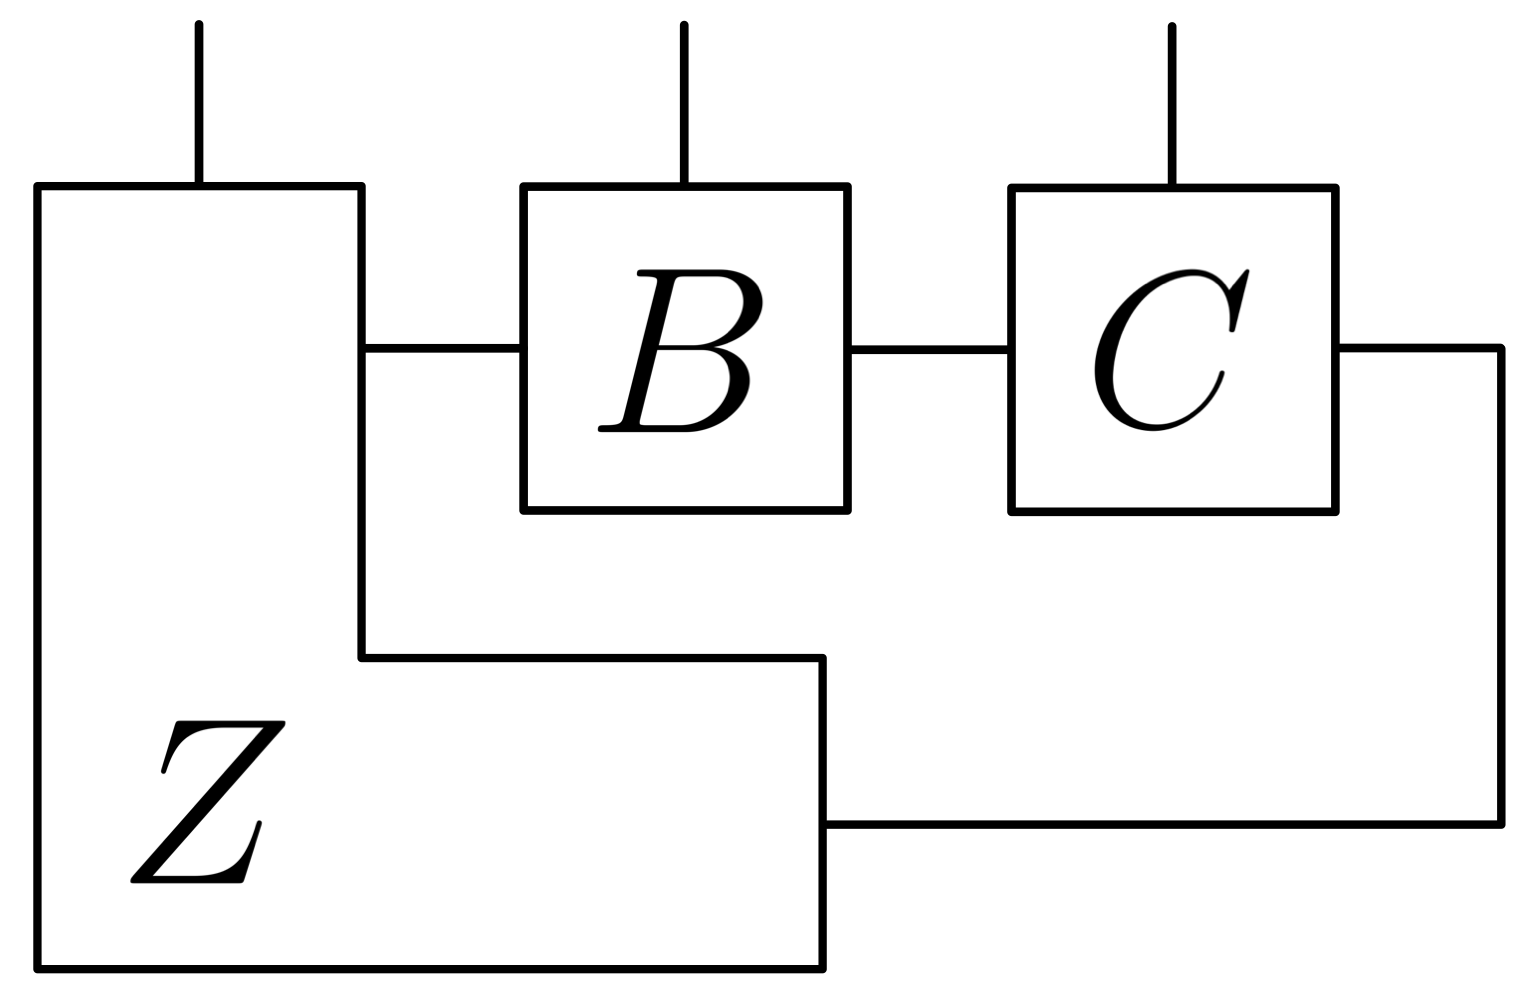
\includegraphics[height=2.2cm]{Z_B_C.png}} \: \middle\vert Z \: \in \mathbb{C}^{d_A \times D \times D} \right\}
\end{equation*}
\begin{equation*}
 	= \left\{ \raisebox{-0.5\height}{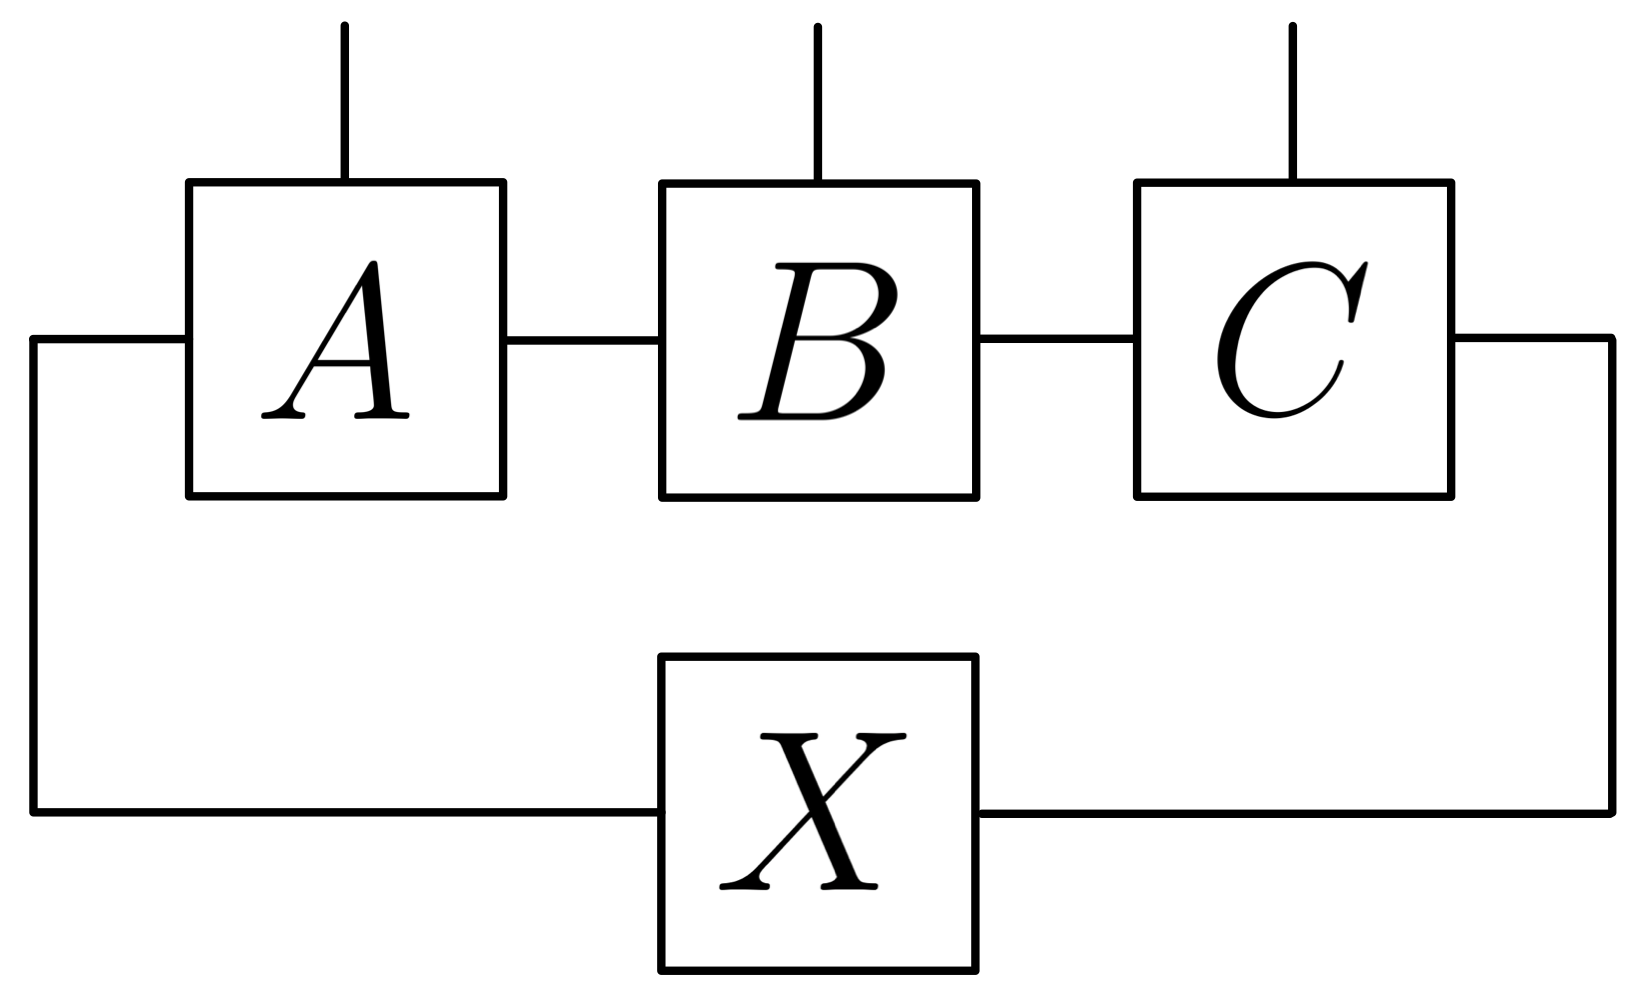
\includegraphics[height=2.2cm]{A_B_C_X.png}} \: \middle\vert \: X \in \mathbb{C}^{D \times D} \right\}.
\end{equation*}
\end{theorem}
% proof
\begin{proof}
Diagrammatic. \cite{cirac2021matrix}
\begin{align}
	& \raisebox{-0.5\height}{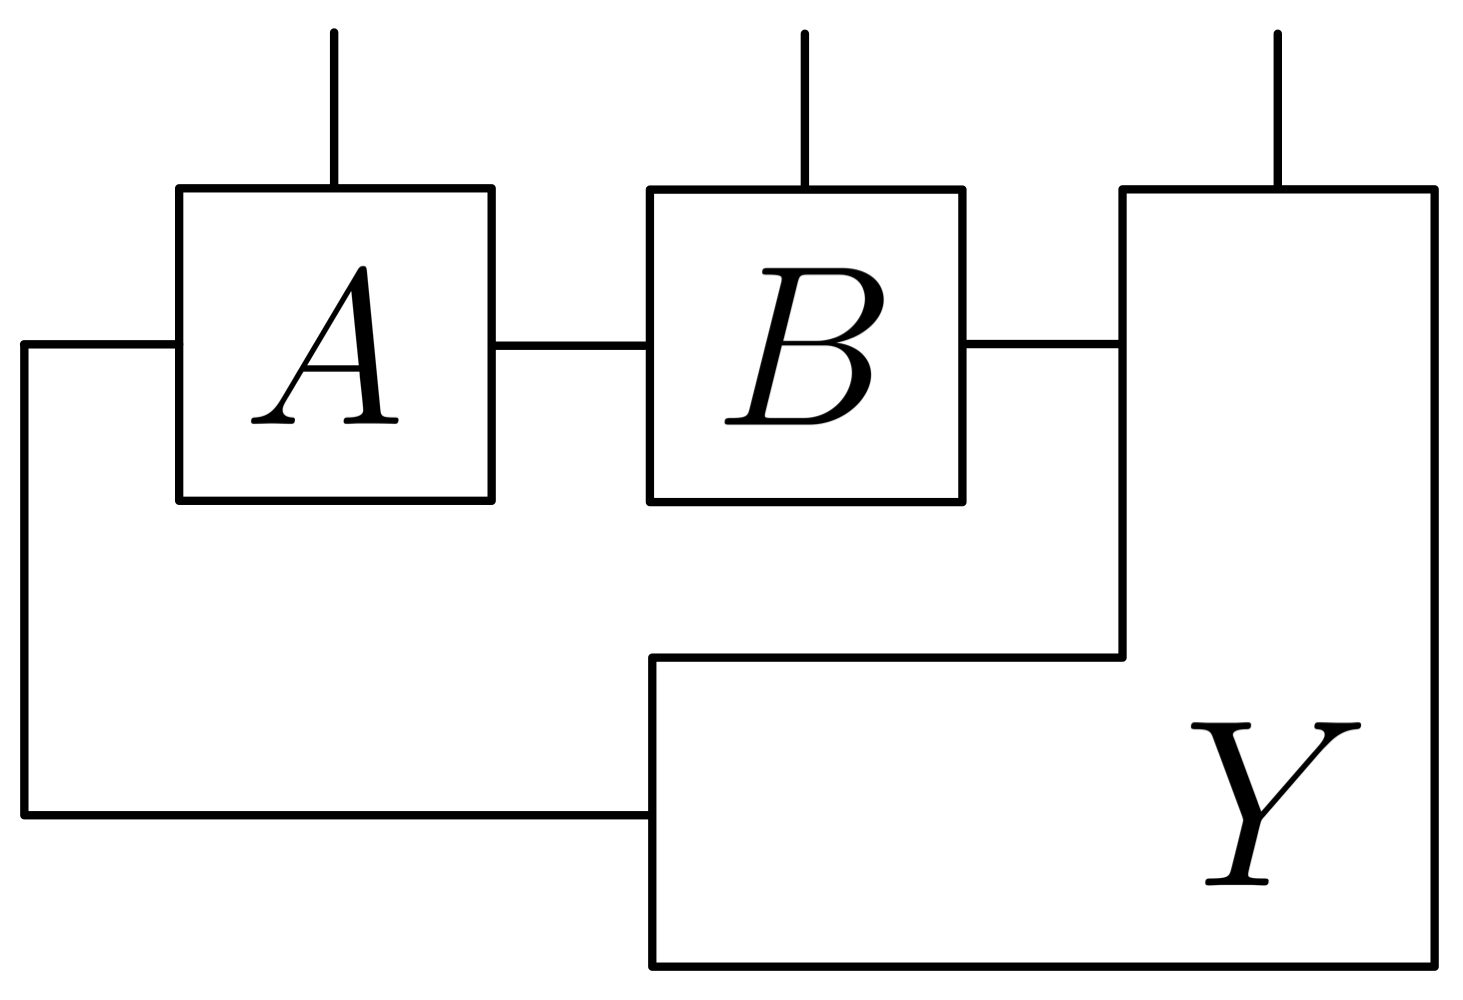
\includegraphics[height=2.2cm]{A_B_Y.png}} \:\: 
	= \:\: \raisebox{-0.5\height}{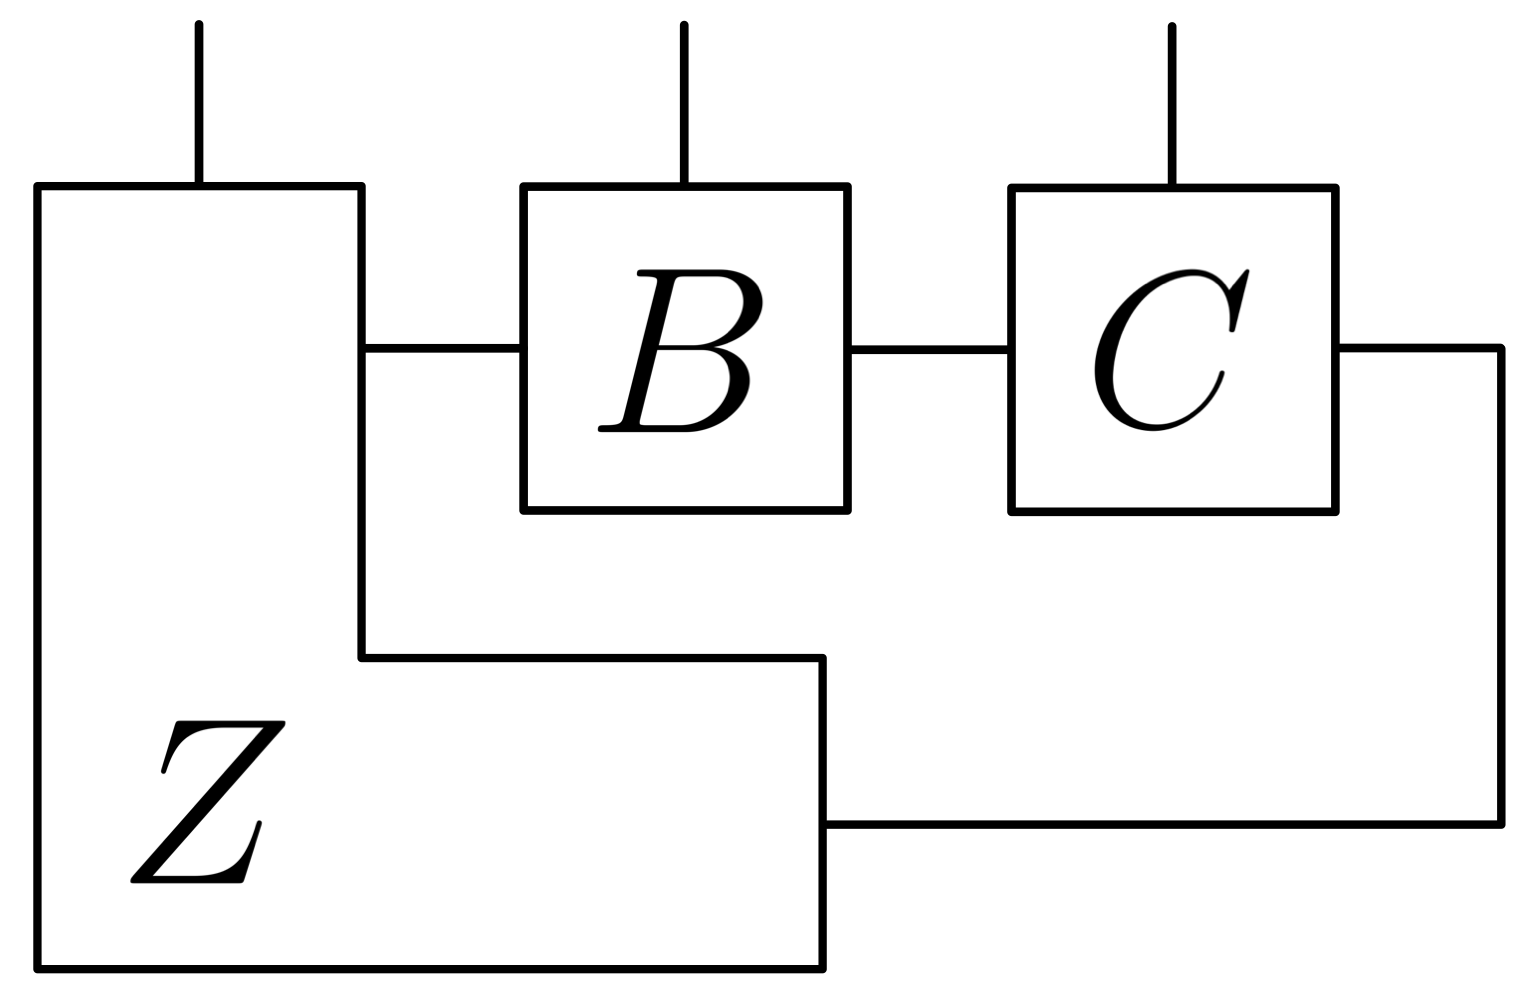
\includegraphics[height=2.2cm]{Z_B_C.png}} \\[0.8em]
	\text{Invert } B \:\:\:\: &
	\raisebox{-0.5\height}{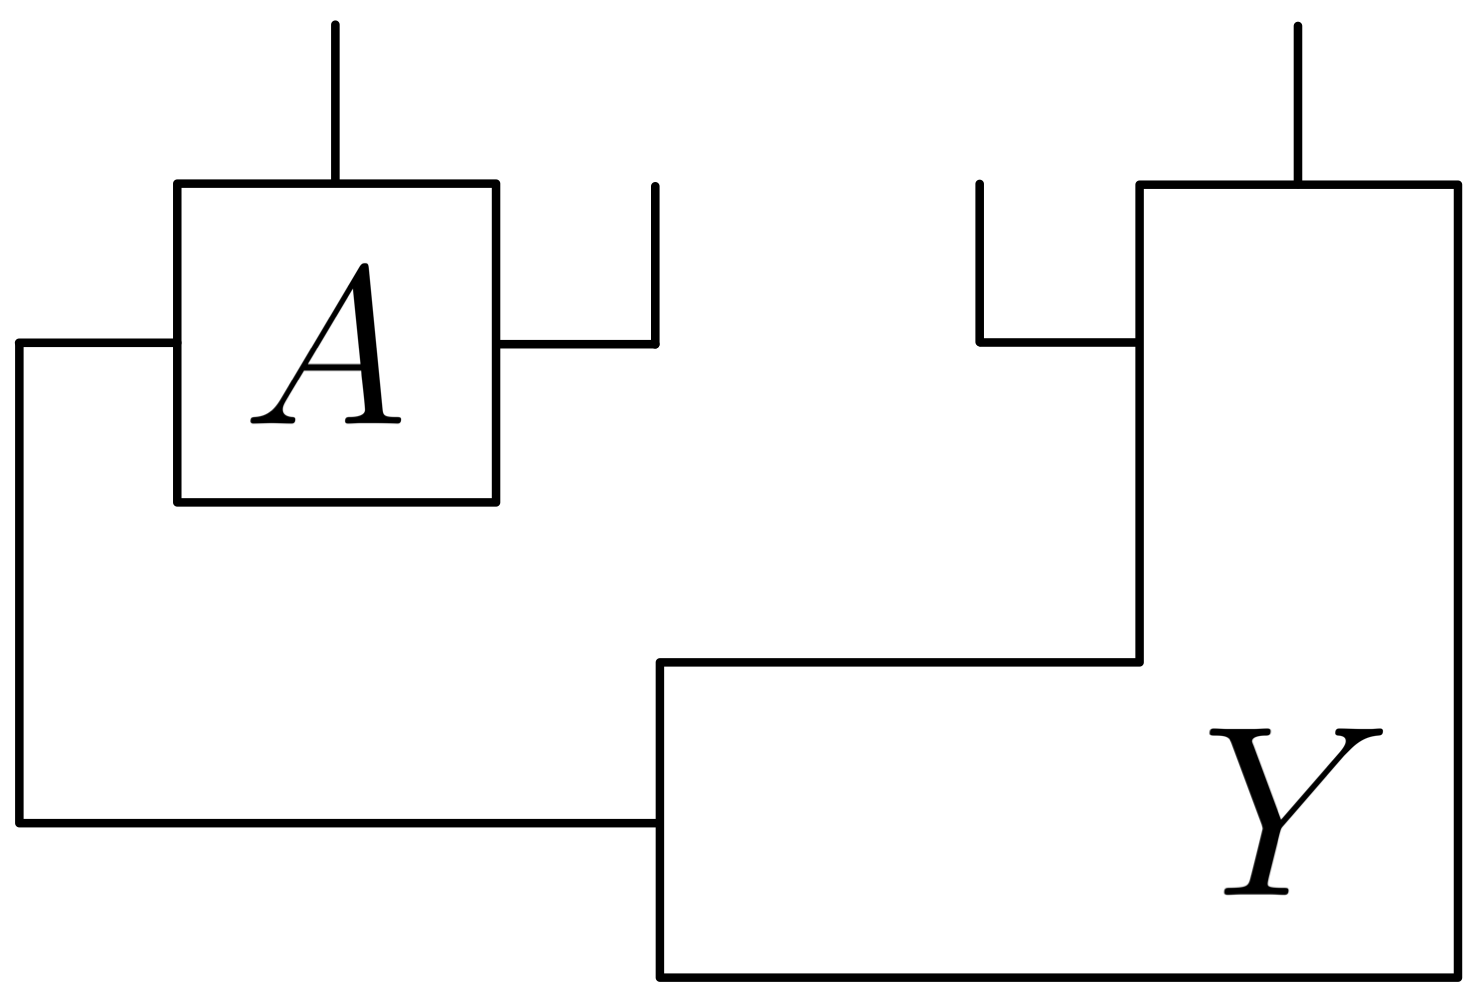
\includegraphics[height=2.2cm]{A_Y.png}} \:\: 
	= \:\: \raisebox{-0.5\height}{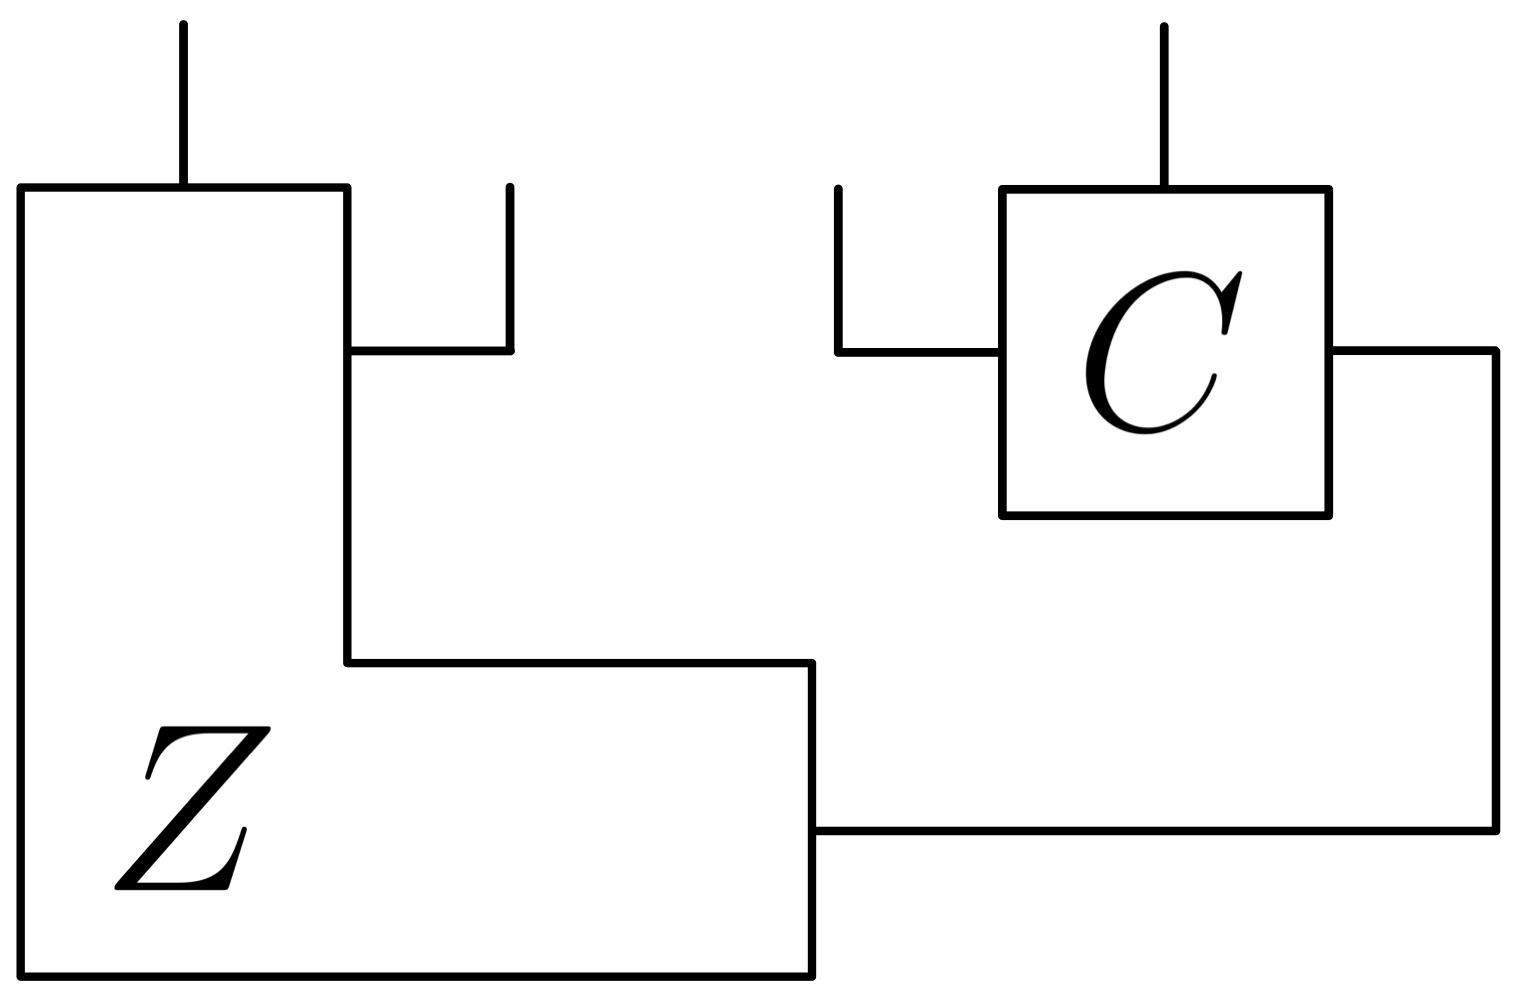
\includegraphics[height=2.2cm]{Z_C.png}} \\[0.8em]
	\text{Re-attach } B \:\:\:\: &
	\raisebox{-0.5\height}{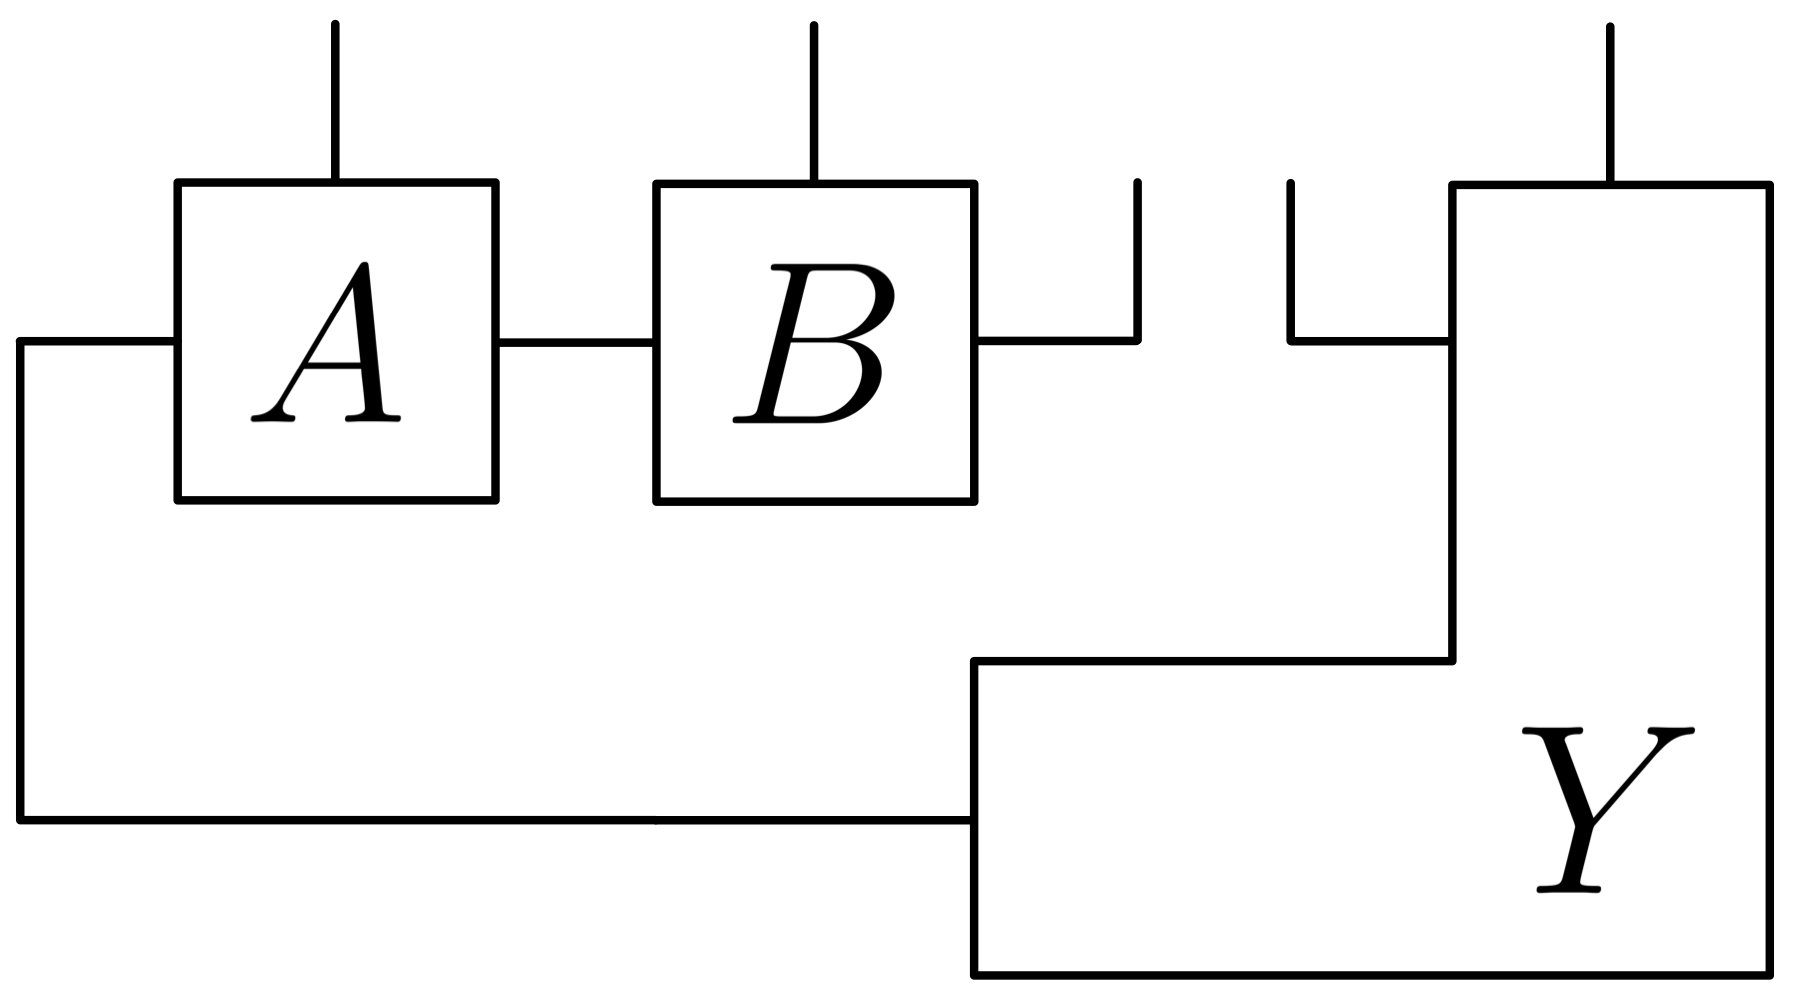
\includegraphics[height=2.2cm]{A_B_Y_2.png}} \:\: 
	= \:\: \raisebox{-0.5\height}{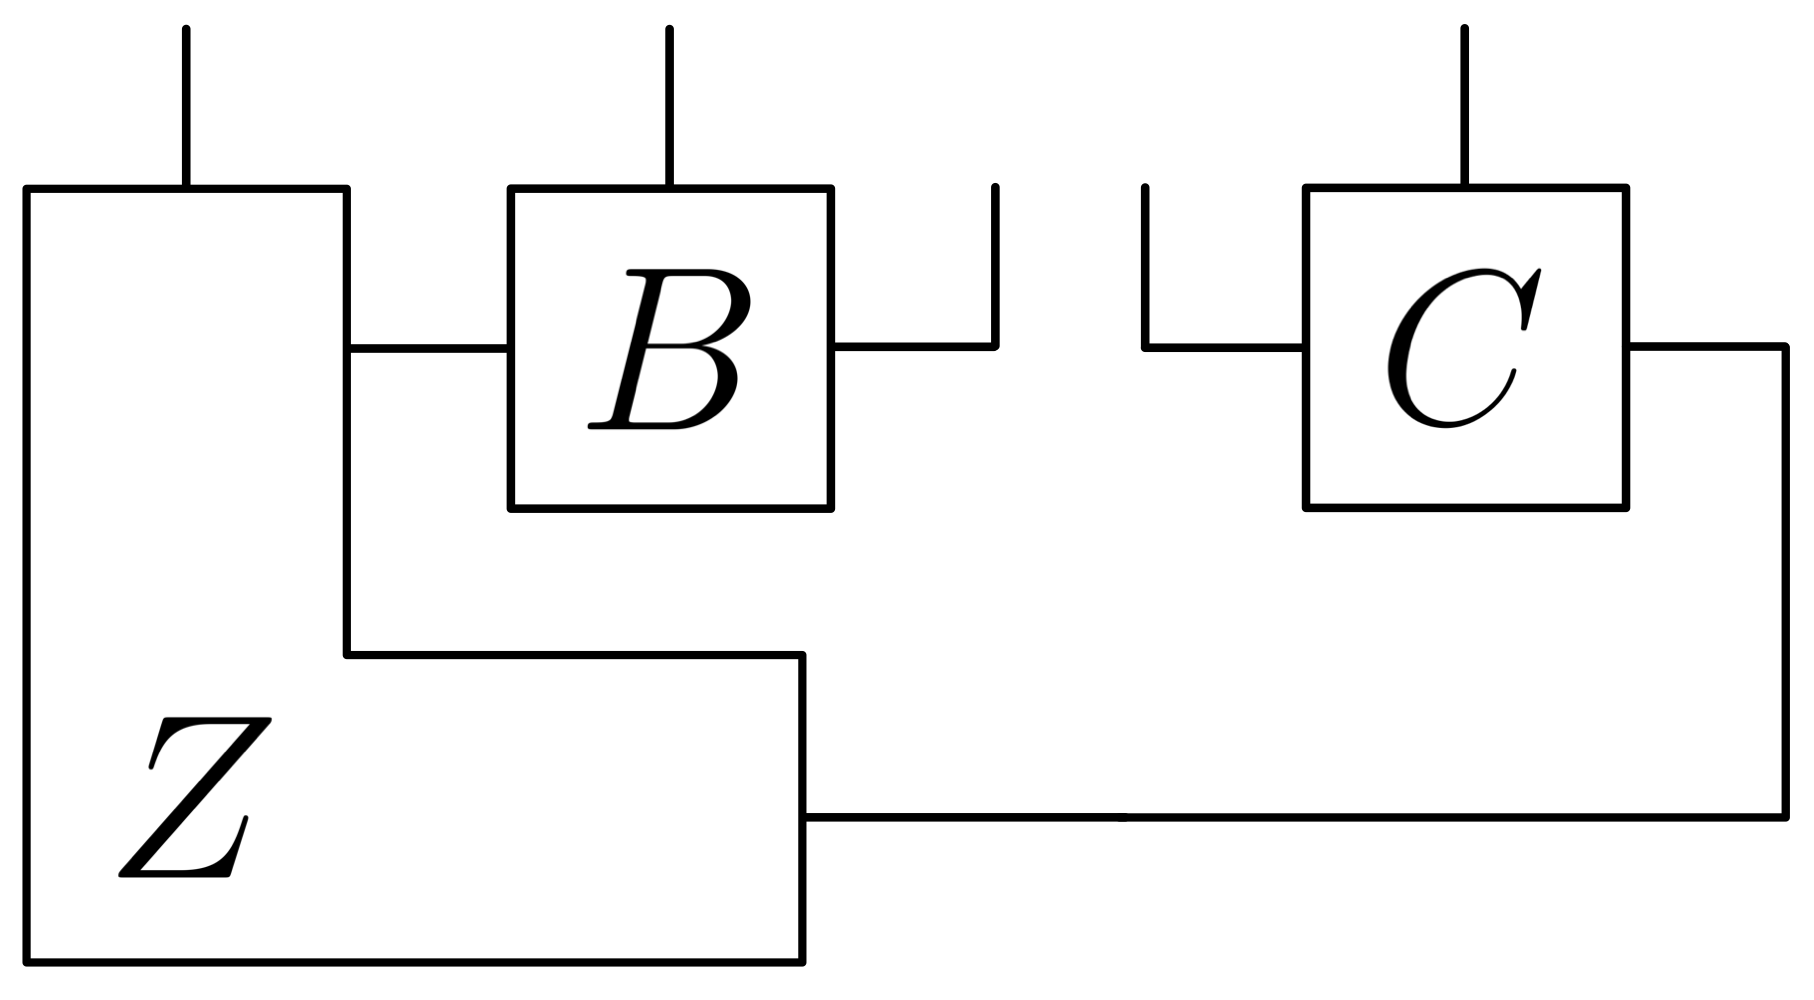
\includegraphics[height=2.2cm]{Z_B_C_2.png}} \\[0.8em]
	\text{Invert } (AB) \:\:\:\: & 
	\raisebox{-0.5\height}{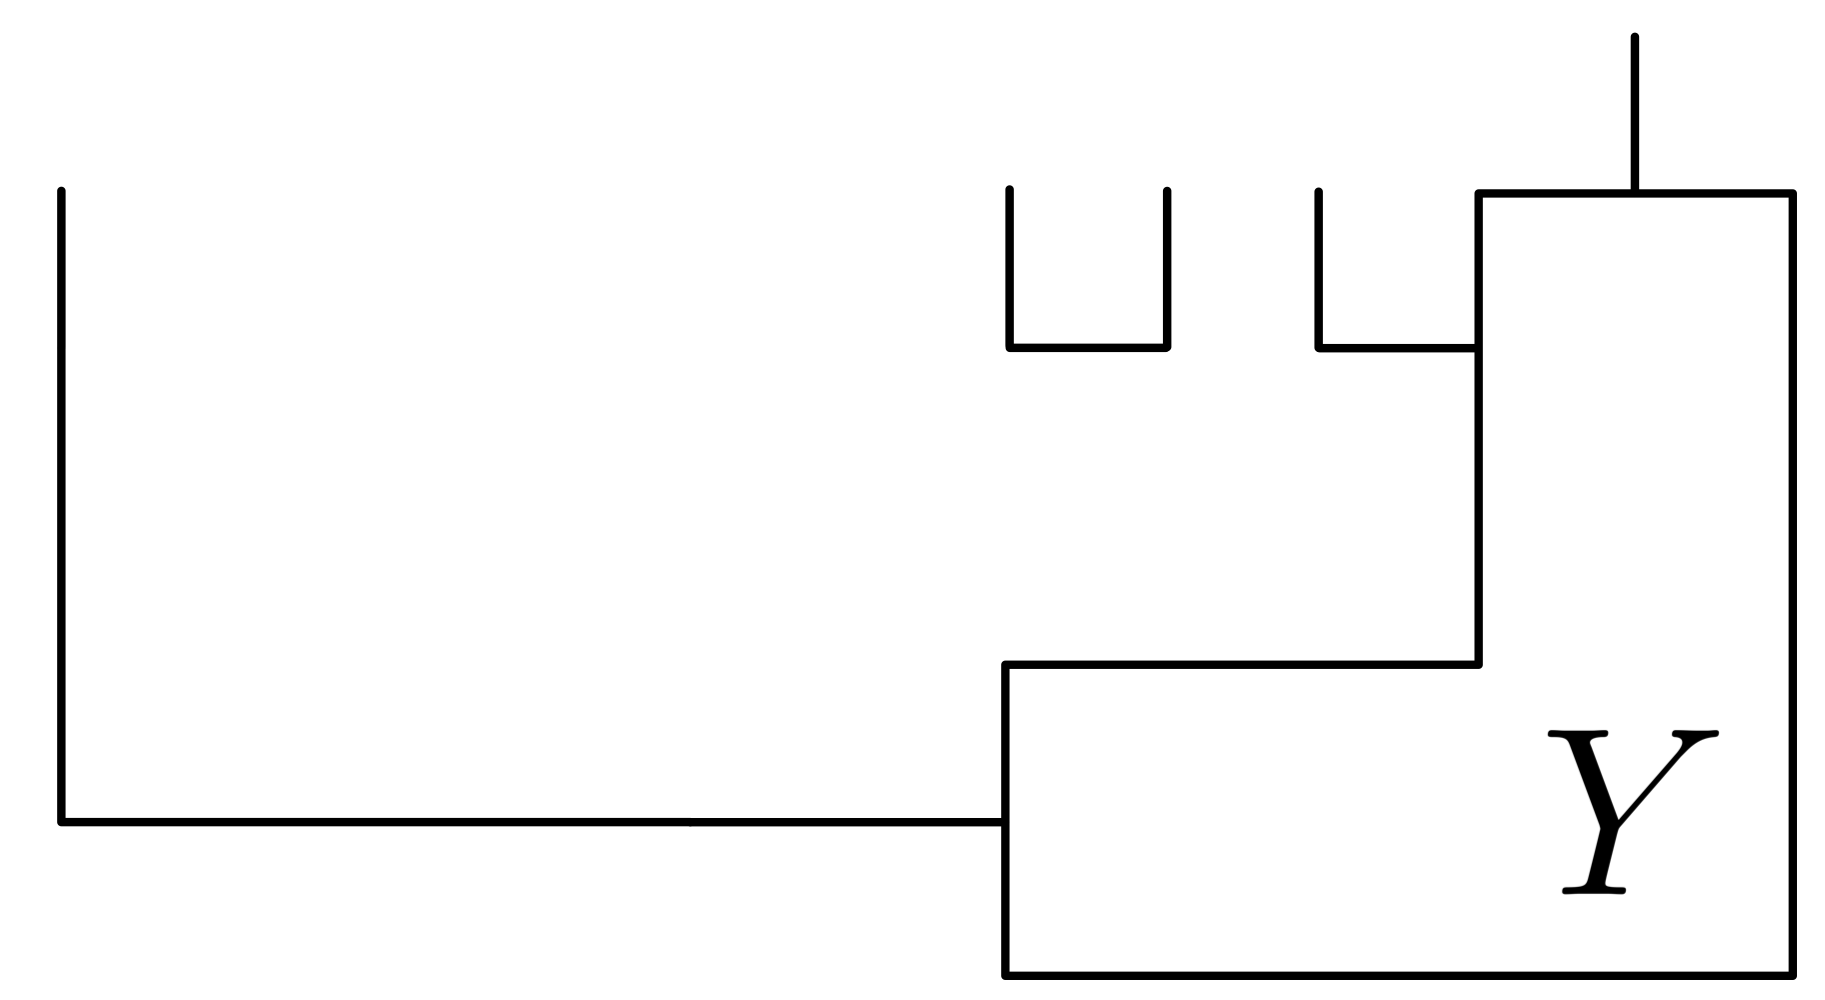
\includegraphics[height=2.2cm]{Y_id.png}} \:\: 
	= \:\: \raisebox{-0.5\height}{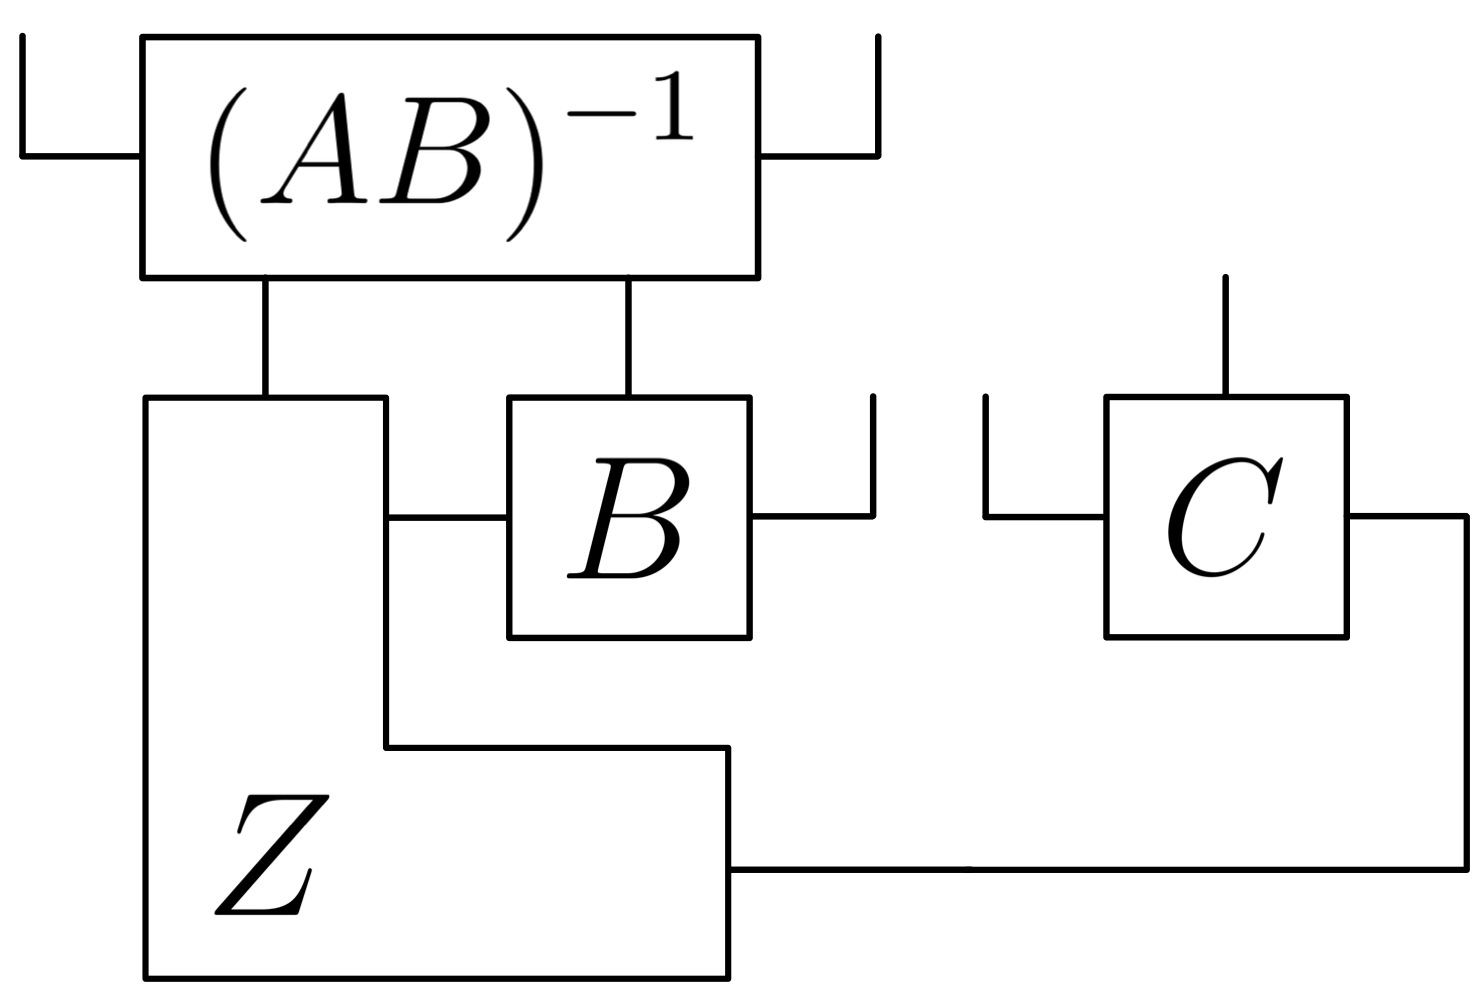
\includegraphics[height=3cm]{Z_B_C_AB_inverse.png}} \\[0.8em]
	\text{Contract} \:\:\:\: &
	\raisebox{-0.5\height}{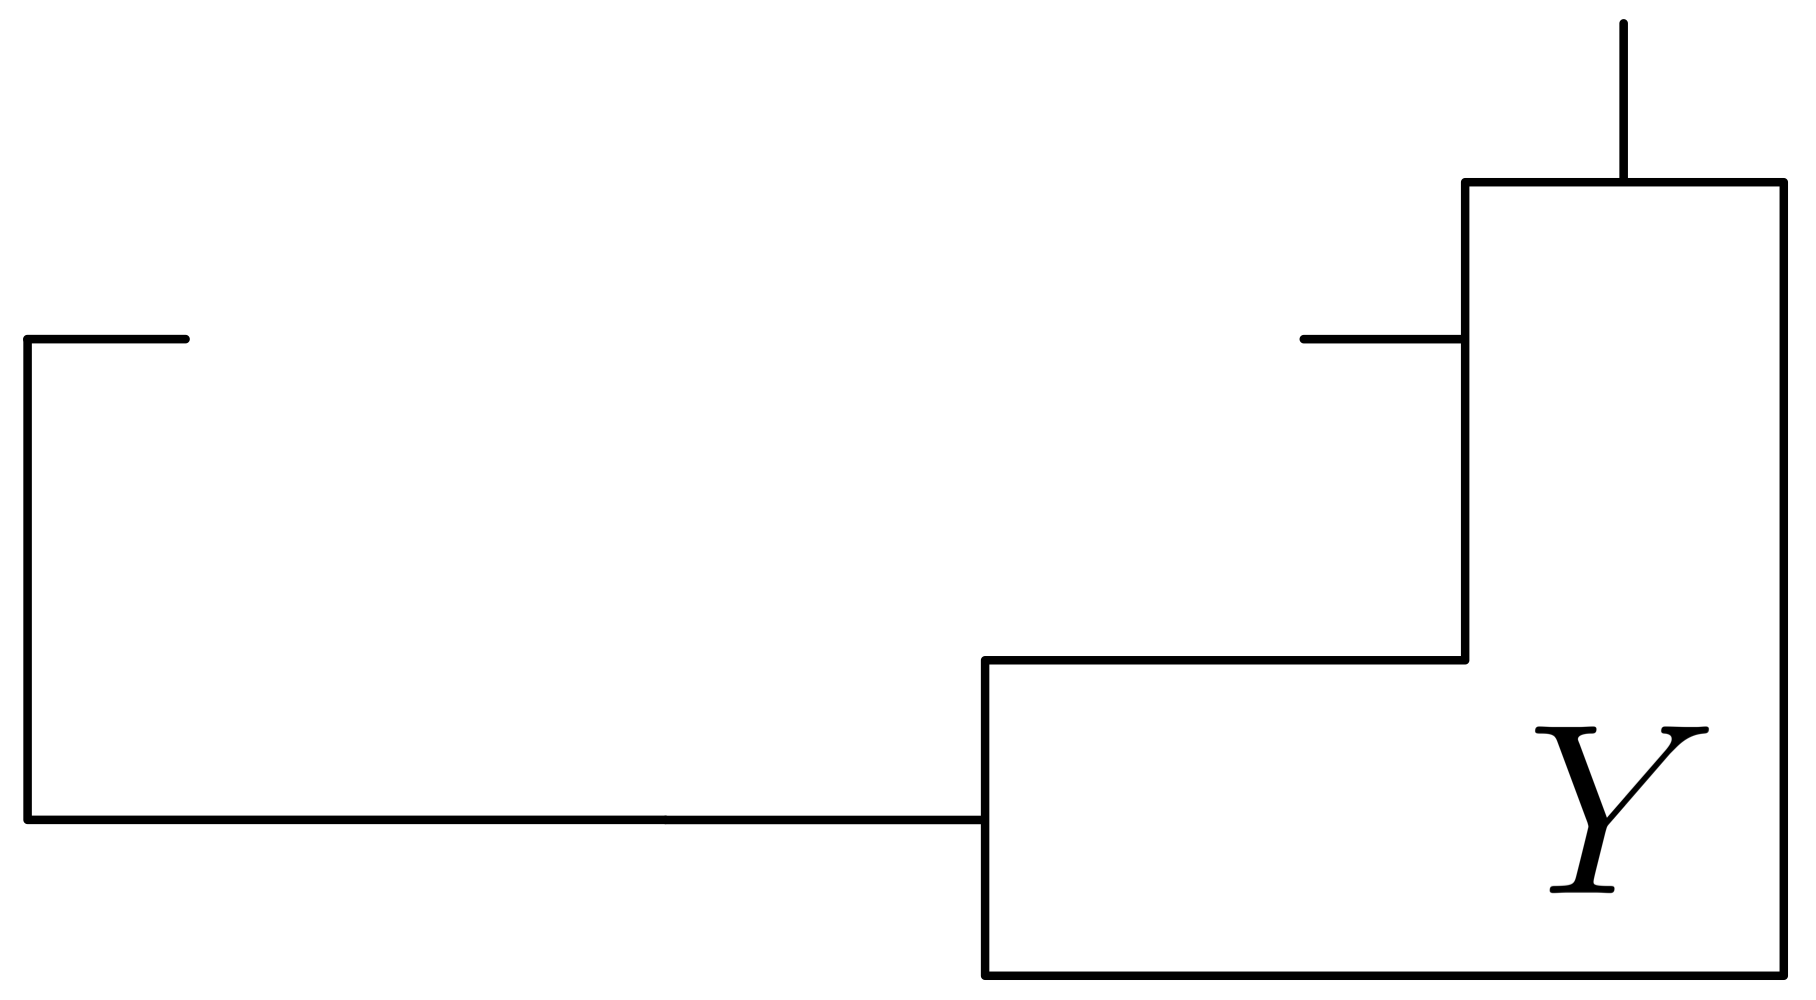
\includegraphics[height=2.2cm]{Y.png}} \:\: 
	= \:\: \raisebox{-0.5\height}{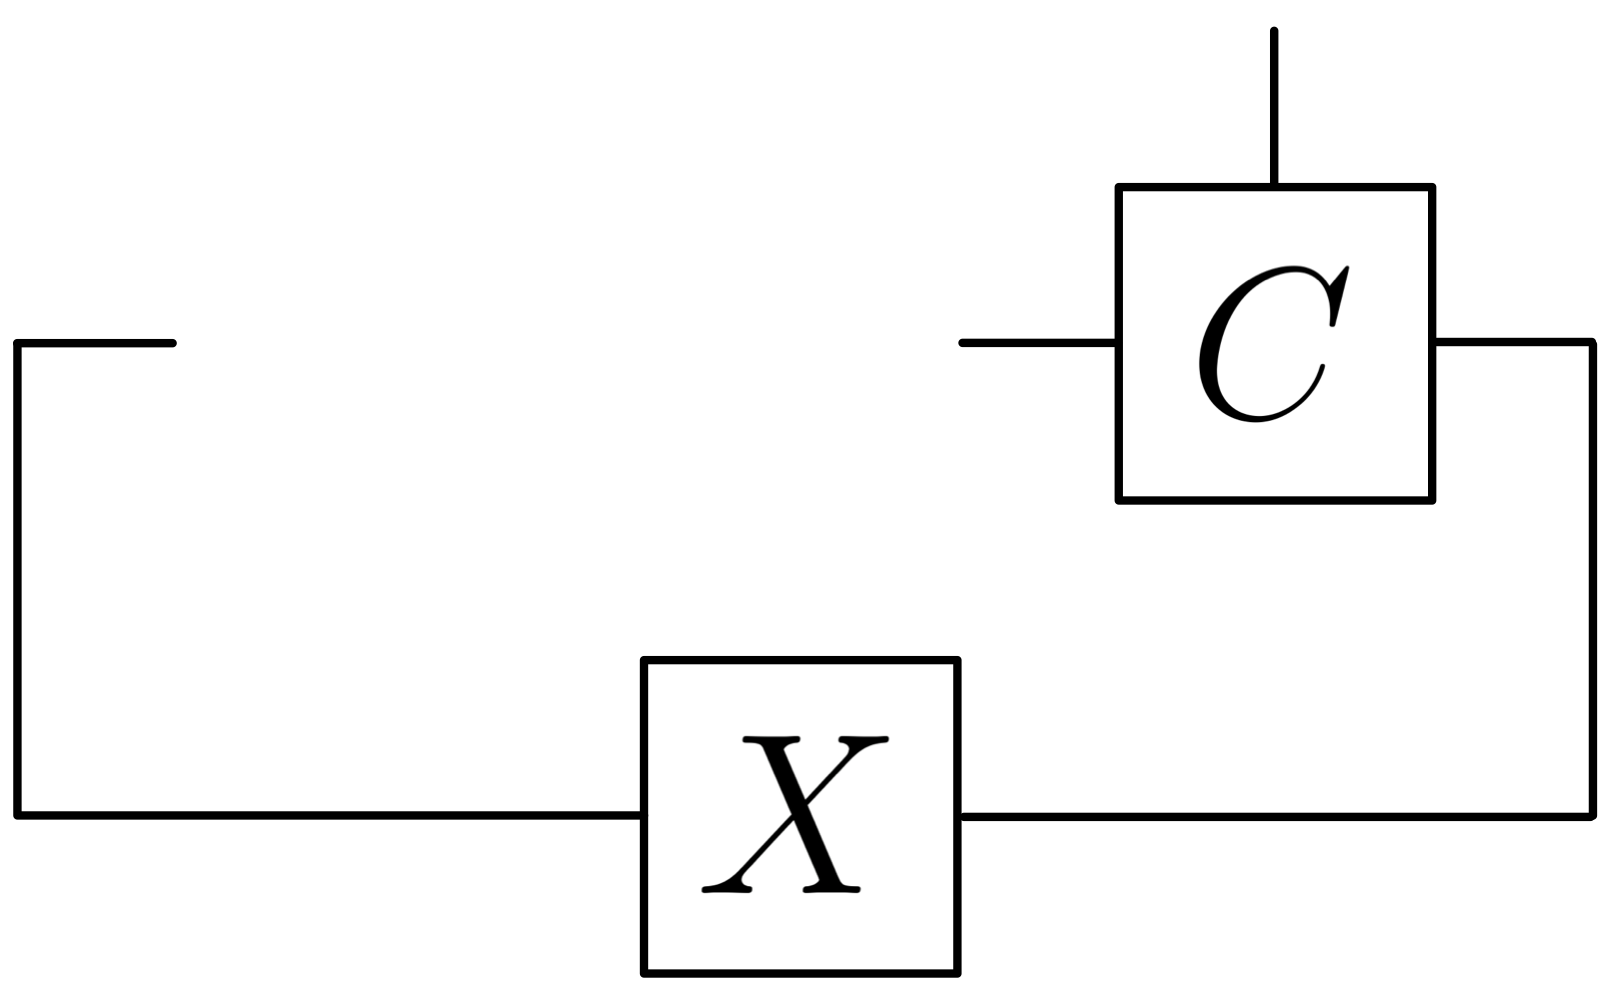
\includegraphics[height=2.2cm]{X_C.png}}
\end{align}
\end{proof}

% closure property
\newpage
\begin{theorem}{Closure property}{closure_property}
Let $A \in \mathbb{C}^{d_A \times D \times D}$ and $B \in \mathbb{C}^{d_B \times D \times D}$ be both invertible. Then
\begin{equation*}
	\left\{ \sum_{s, k} \tr[X A^s B^k] \ket{s, k} \mid X \in \mathbb{C}^{D \times D} \right\} 
	\cap 
	\left\{ \sum_{s, k} \tr[A^s Y B^k] \ket{s, k} \mid Y \in \mathbb{C}^{D \times D} \right\} \vspace{-1em}
\end{equation*}
\begin{equation}
	= \mathrm{span}\left\{\sum_{s, k} \tr[A^s B^k] \ket{s, k} \right\}.
\end{equation}
\begin{equation*}
	\left\{ \raisebox{-0.5\height}{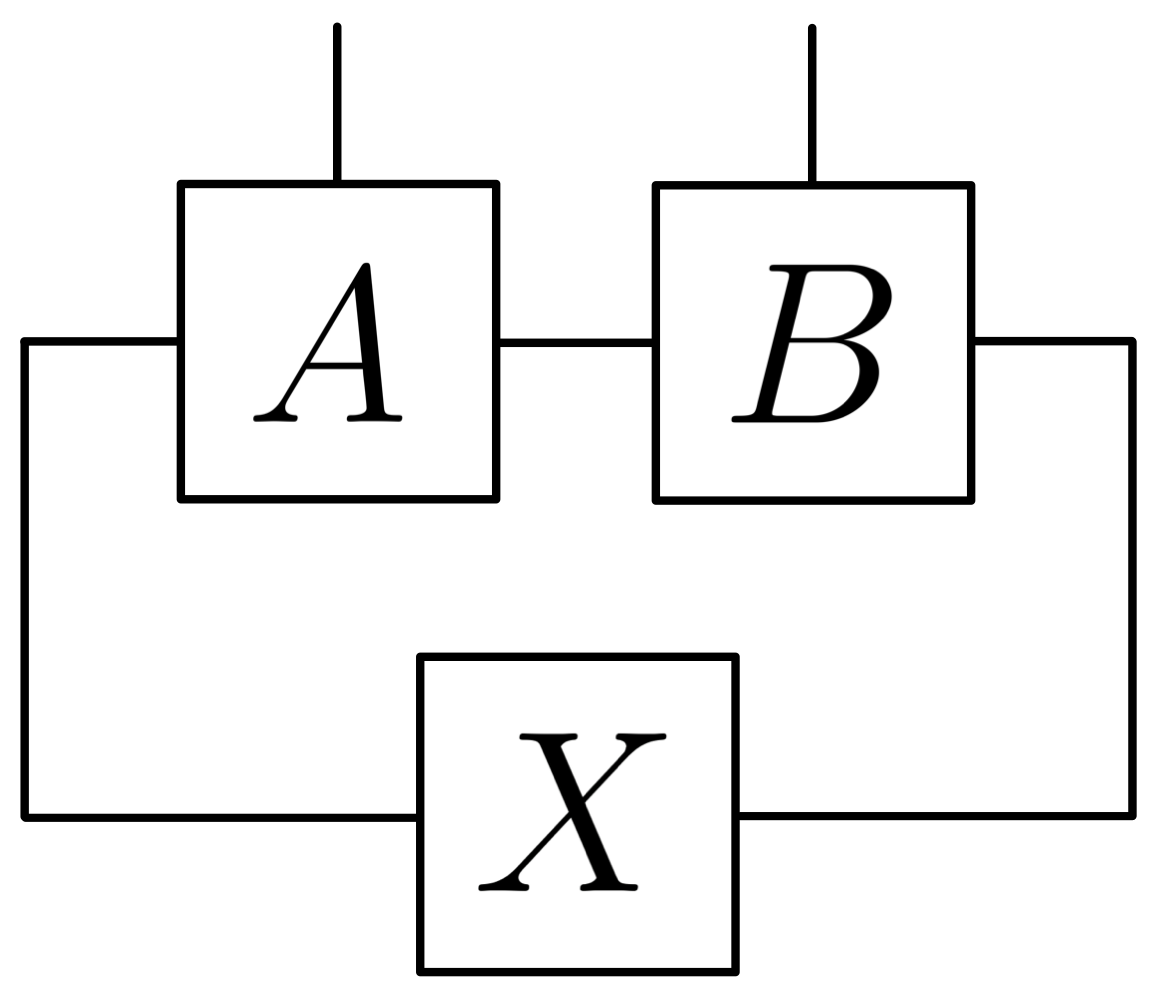
\includegraphics[height=2.2cm]{X_A_B.png}} \: \middle\vert \: X \in \mathbb{C}^{D \times D} \right\} \:\:
	\cap 
	\:\: \left\{ \raisebox{-0.5\height}{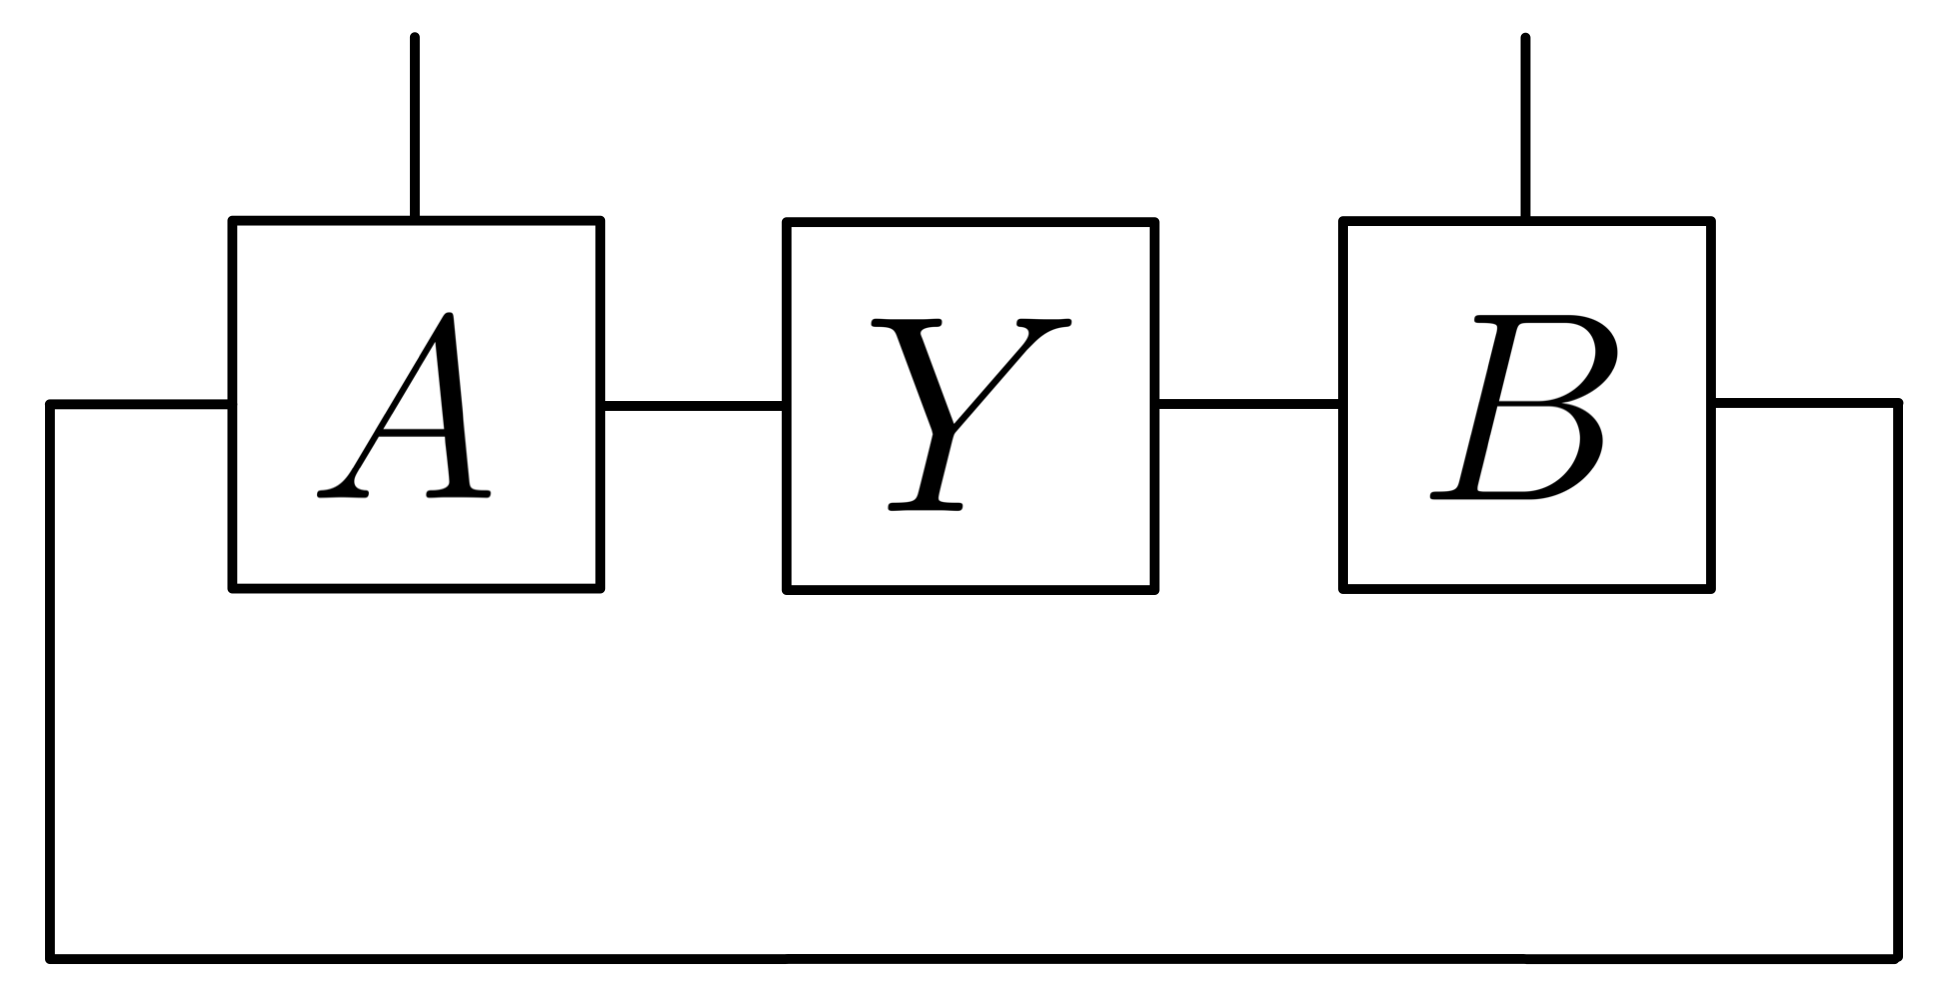
\includegraphics[height=1.9cm]{A_Y_B.png}} \: \middle\vert \: Y  \in \mathbb{C}^{D \times D} \right\}
\end{equation*}
\begin{equation*}
 	= \left\{ \alpha \cdot \raisebox{-0.5\height}{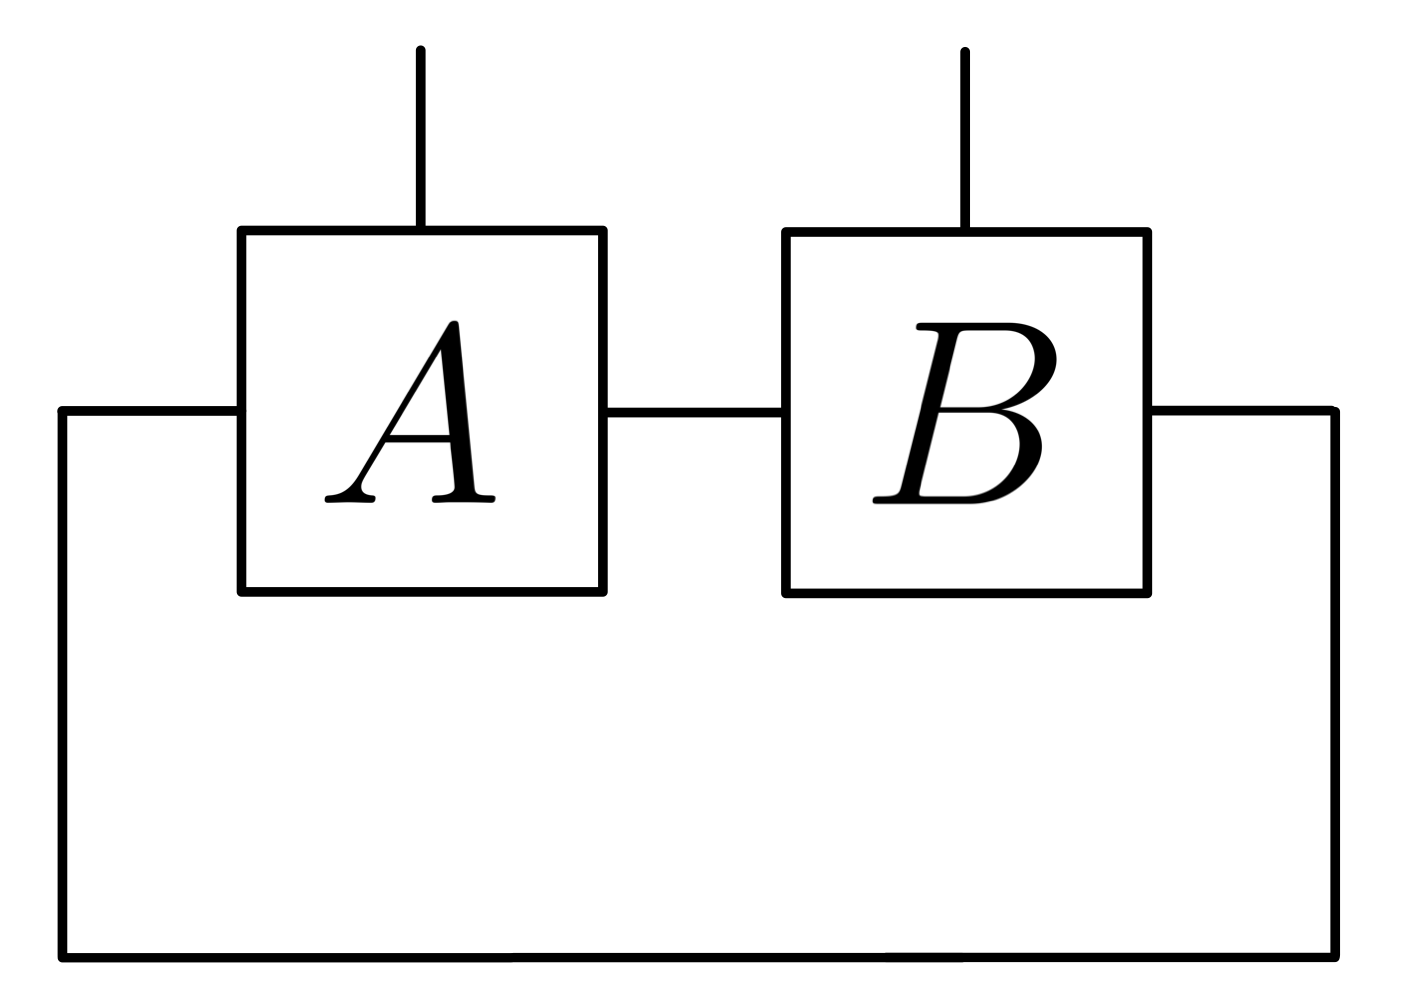
\includegraphics[height=1.9cm]{A_B.png}} \: \middle\vert \: \alpha \in \mathbb{C} \right\}.
\end{equation*}
\end{theorem}
% proof
\begin{proof}
Diagrammatic. \cite{schuch2010peps}
\begin{align}
	& \raisebox{-0.5\height}{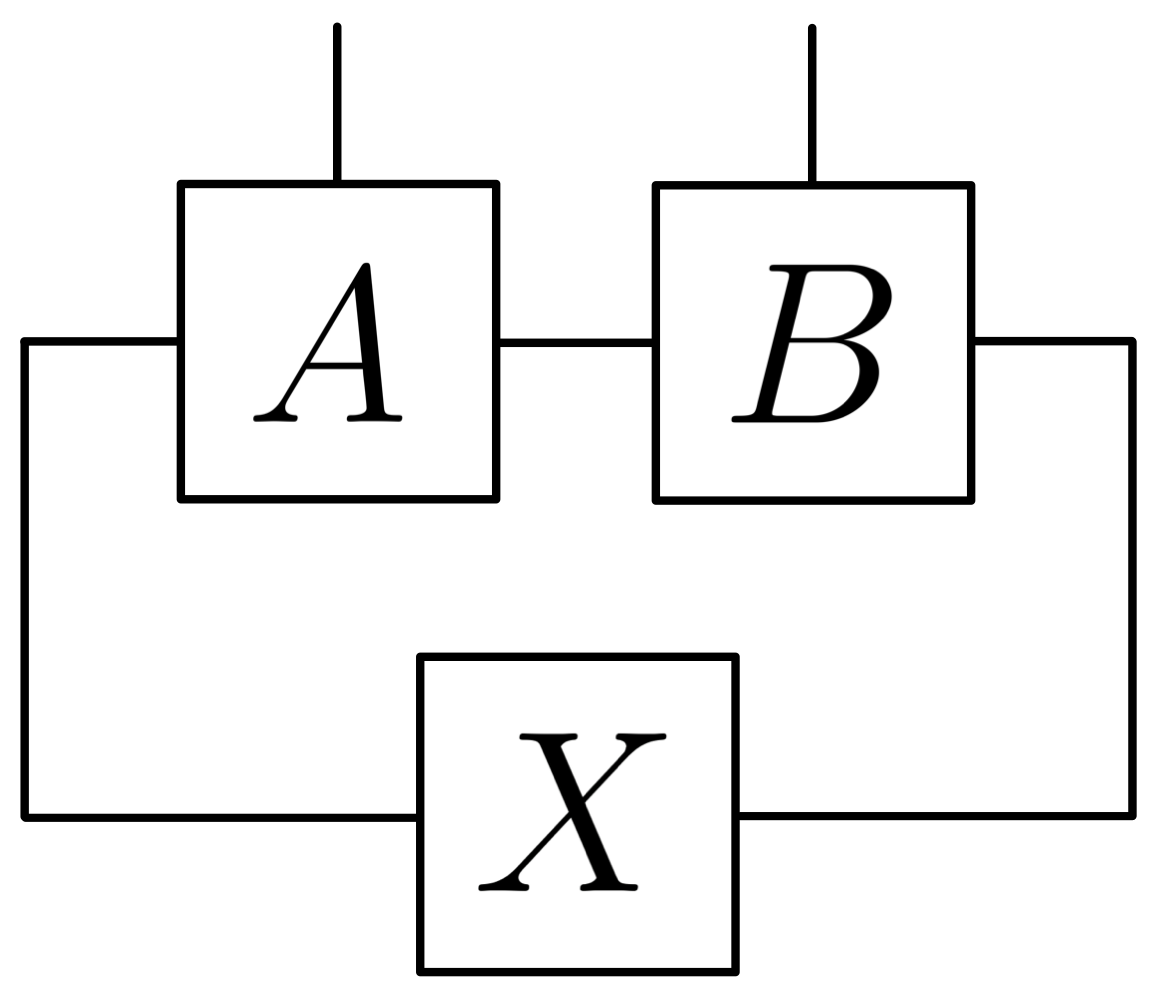
\includegraphics[height=2.2cm]{X_A_B.png}} \:\: 
	= \:\: \raisebox{-0.4\height}{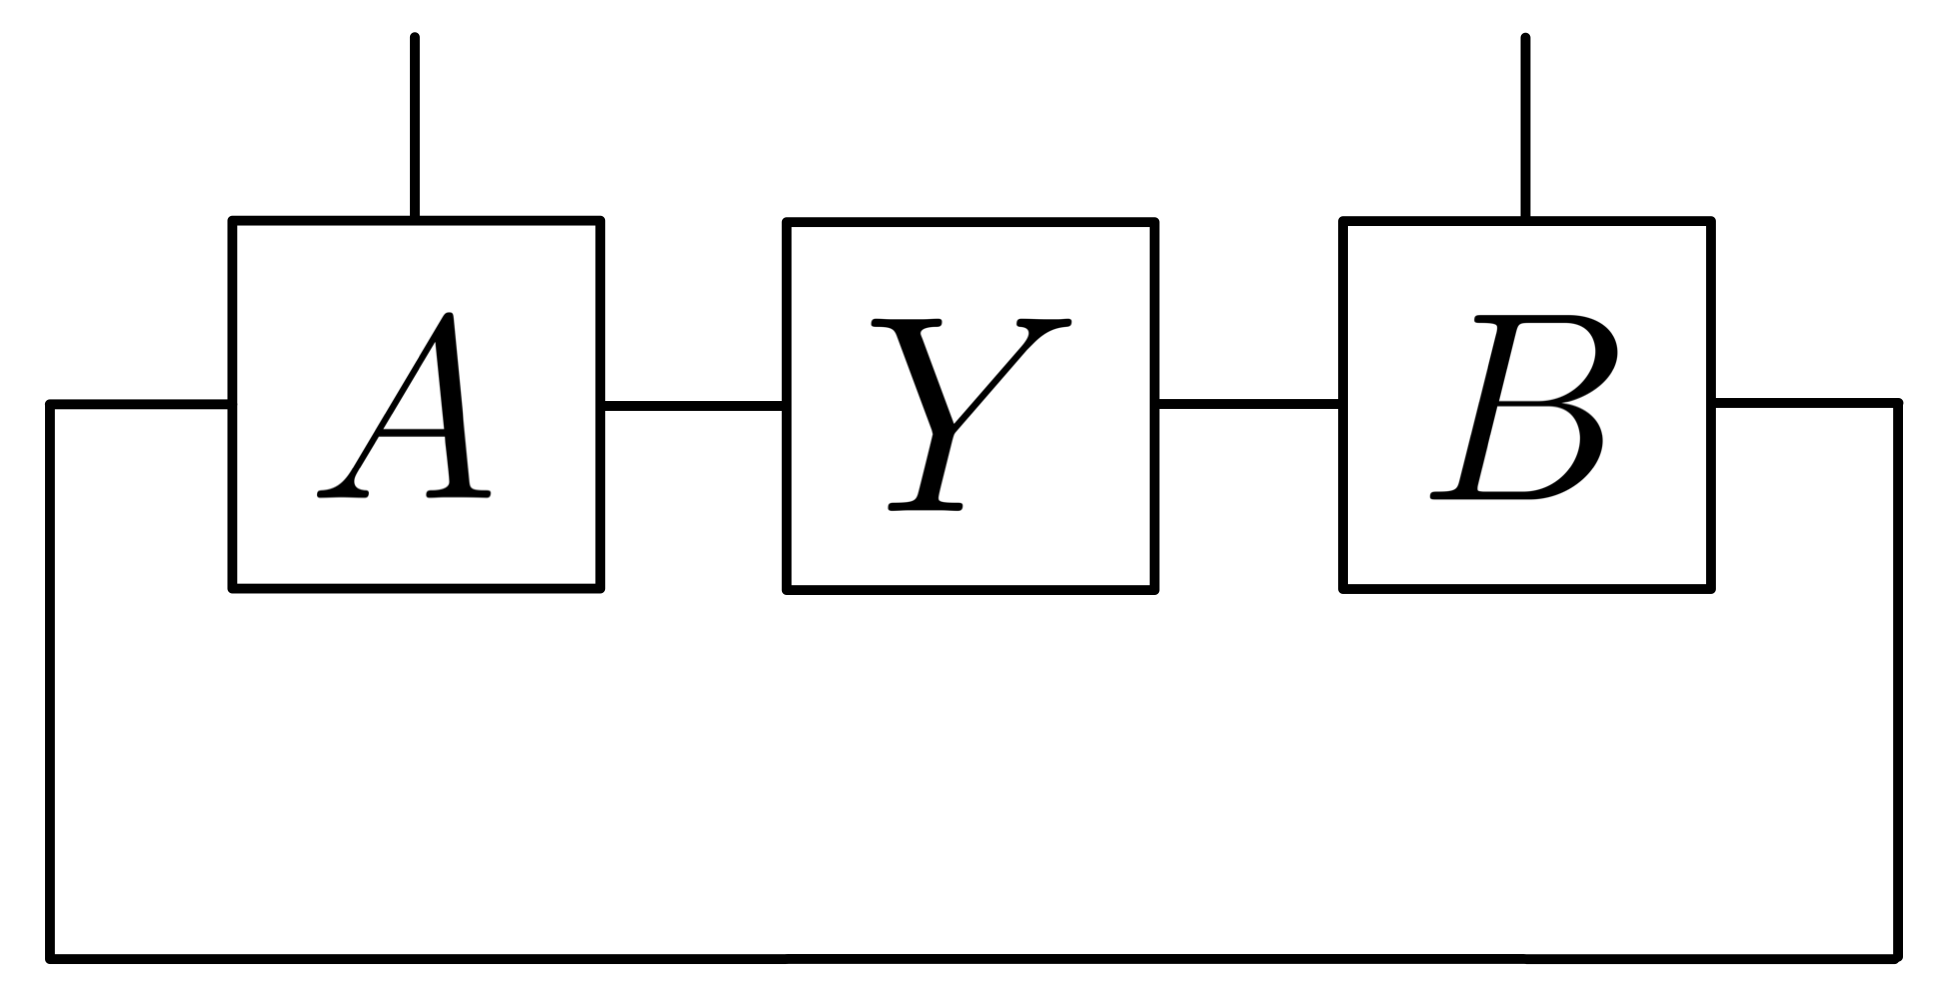
\includegraphics[height=1.9cm]{A_Y_B.png}} \\[0.8em]
	\text{Invert } A, B \:\:\:\: &
	\raisebox{-0.5\height}{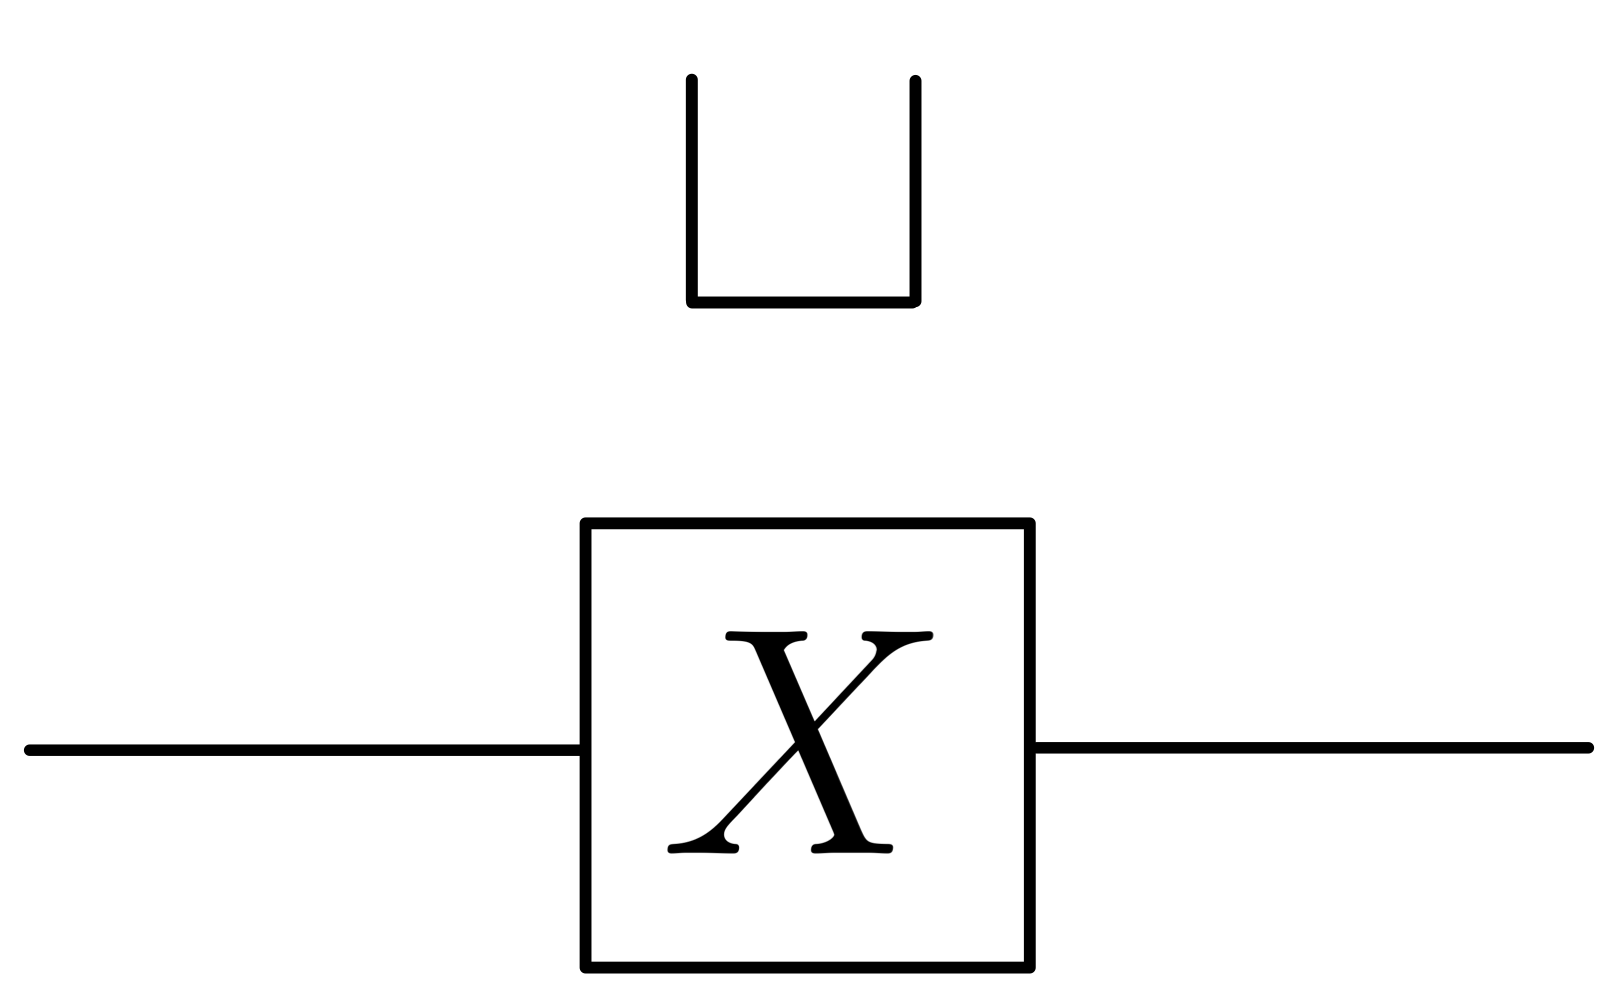
\includegraphics[height=1.6cm]{X_id.png}} \:\: 
	= \:\: \raisebox{-0.42\height}{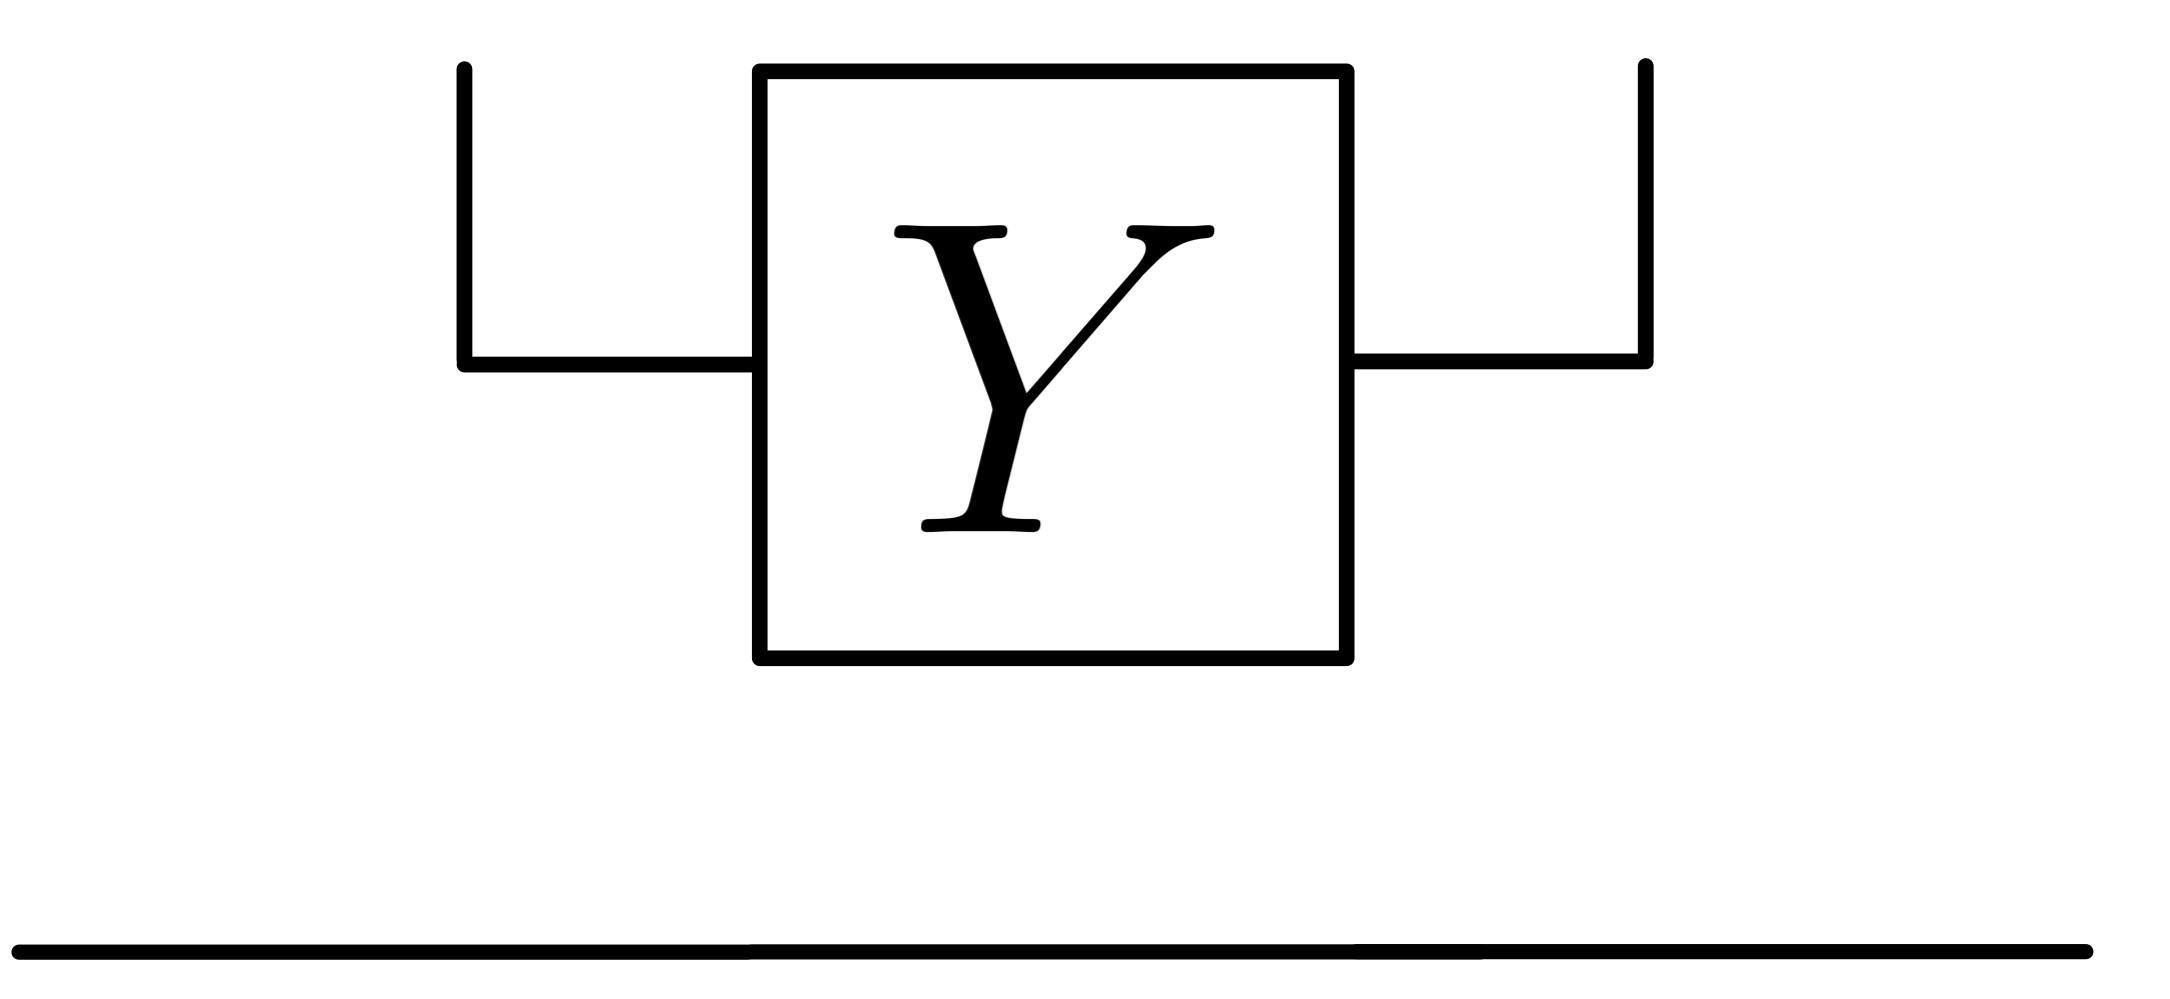
\includegraphics[height=1.2cm]{id_Y.png}} \\[0.8em]
	\text{Contract} \:\:\:\: & 
	\raisebox{-0.35\height}{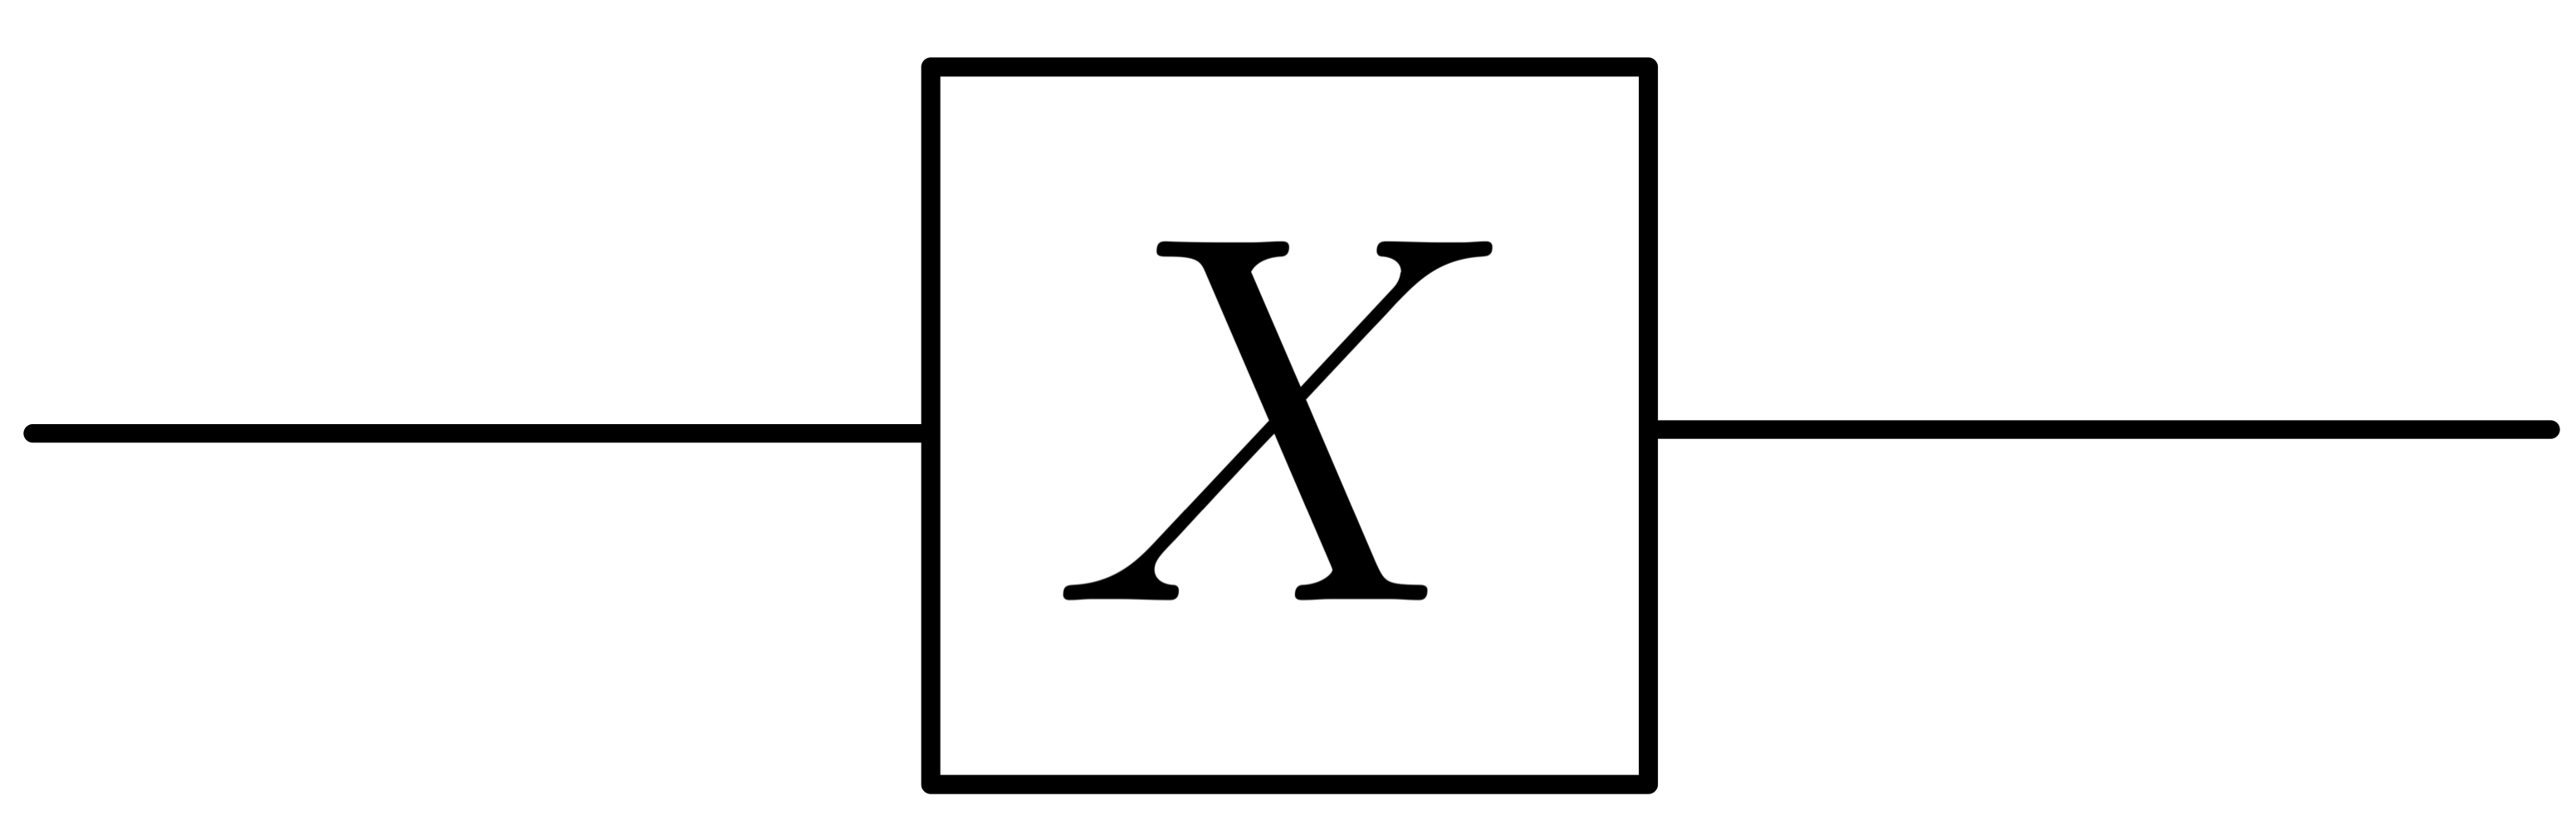
\includegraphics[height=0.83cm]{X.png}} \:\: 
	= \:\: \frac{1}{D} \: \raisebox{0\height}{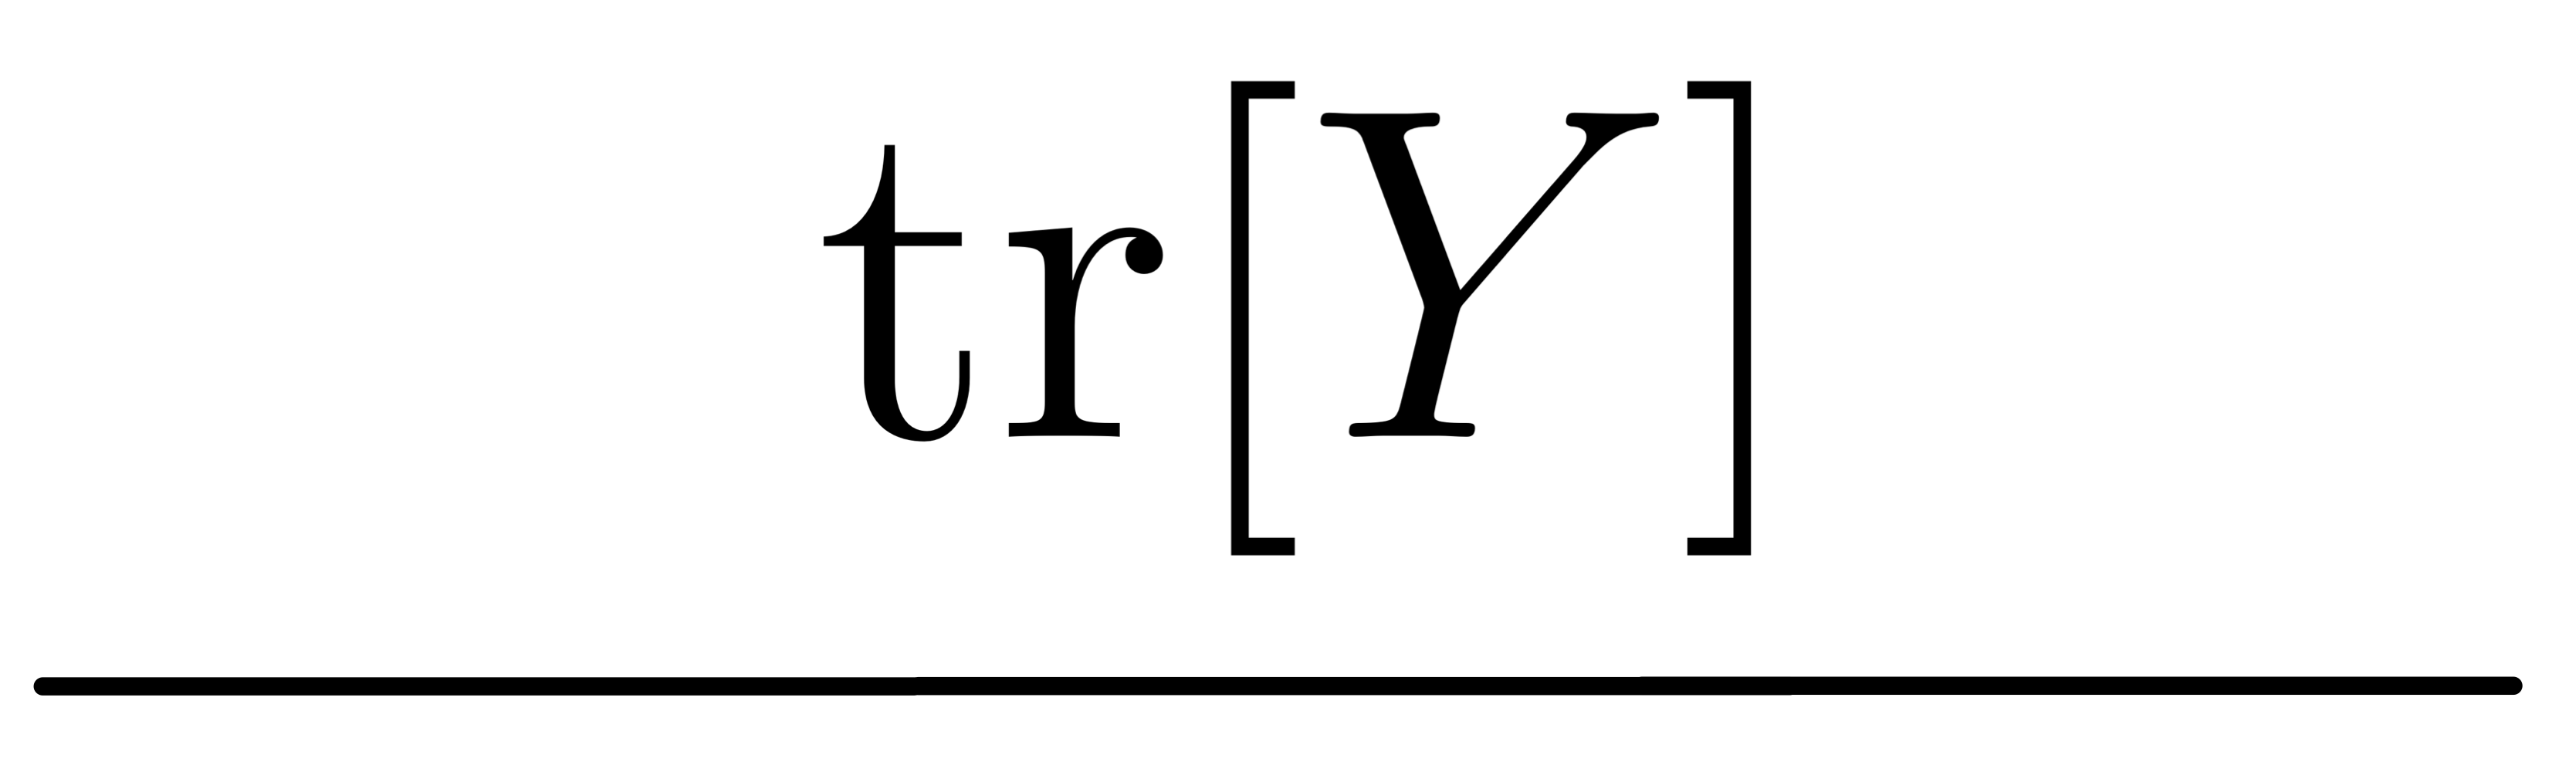
\includegraphics[height=0.8cm]{id_trY.png}}
\end{align}
\end{proof}

% unique ground state 
\begin{theorem}{Unique ground state}{unique_ground_state}
Let $A \in \mathbb{C}^{d \times D \times D}$ be an invertible tensor with injectivity length $L_0$. For $L \geq L_0+1$ and $N \geq L+L_0$, $\ket{\psi(A,N)}$ is the unique ground state of the corresponding parent Hamiltonian:
\begin{equation}
	\mathrm{ker}(H) = \mathrm{span}\left\{\ket{\psi(A,N)}\right\}.
\end{equation}

\end{theorem}
% proof
\begin{proof}
By theorem \ref{thm:frustration_free} the ground space of the parent Hamiltonian is given by
\begin{equation}
	\mathrm{ker}(H) = \bigcap_{n=1}^N \mathrm{ker}(h_n) \:\:\text{with}\:\: \mathrm{ker}(h_n) = \mathbb{C}^{d^{n-1}} \otimes \mathcal{G}_{A^L} \otimes \mathbb{C}^{d^{N-L-n+1}}.
\end{equation}
We split the Hamiltonian into two sums defined by
\begin{align}
	H_{\mathrm{left}} &\coloneqq h_1 + \ldots + h_{L-1} + \frac{1}{2}(h_L + \ldots + h_{N-L+1}), \label{eq_H_left} \\ 
	H_{\mathrm{right}} &\coloneqq \frac{1}{2}(h_L + \ldots + h_{N-L+1}) + h_{N-L+2} + \ldots + h_{N}. \label{eq_H_right}
\end{align}
$N-L$ applications of the intersection property \ref{thm:intersection_property} yield:
\begin{equation*}
	\mathrm{ker}(H_{\mathrm{left}}) = \underbrace{\underbrace{\underbrace{(\mathcal{G}_{AA^{L-1}} \otimes \mathbb{C}^d \otimes \mathbb{C}^{d^{N-L-1}}) \cap (\mathbb{C}^d \otimes \mathcal{G}_{A^{L-1}A} \otimes \mathbb{C}^{d^{N-L-1}})}_{= \mathcal{G}_{A^2A^{L-1}} \otimes \mathbb{C}^d \otimes \mathbb{C}^{d^{N-L-2}}} \cap\: (\mathbb{C}^{d^2} \otimes \mathcal{G}_{A^{L-1}A} \otimes \mathbb{C}^{d^{N-L-2}})}_{\begin{array}{c} = \mathcal{G}_{A^3A^{L-1}} \otimes \mathbb{C}^d \otimes \mathbb{C}^{d^{N-L-3}} \\ \vdots \end{array}} \cap\: \ldots }_{= \mathcal{G}_{A^N}} 
\end{equation*}
We do the same for $H_{\mathrm{right}}$ to get
\begin{align}
	\mathrm{ker}(H_{\mathrm{left}}) &= \left\{ \sum_{s_1, \ldots, s_N} \tr[X A^{s_1} \cdots A^{s_N}] \ket{s_1 \ldots s_N} \middle\vert X \in \mathbb{C}^{D \times D} \right\}, \\
	\mathrm{ker}(H_{\mathrm{right}}) &= \left\{ \sum_{s_1, \ldots, s_N} \tr[A^{s_1} \cdots A^{s_{L-1}} Y A^{s_L} \cdots A^{s_N}] \ket{s_1 \ldots s_N} \middle\vert Y \in \mathbb{C}^{D \times D} \right\}.	
\end{align}
After one application of the closure property \ref{thm:closure_property} we end up with
\begin{align}
\begin{split}
	\mathrm{ker}(H) &= \mathrm{ker}(H_{\mathrm{left}}) \cap \mathrm{ker}(H_{\mathrm{right}}) \\
	&= \mathrm{span} \left\{ \sum_{s_1, \ldots, s_N} \tr[A^{s_1} \cdots A^{s_N}] \ket{s_1 \ldots s_N} \right\} 
	= \mathrm{span}\left\{\ket{\psi(A,N)}\right\}.
\end{split}
\end{align}
In addition it can be proven that the parent Hamiltonian has a finite energy gap $\Delta > 0$ above the ground state. \cite{perez2007matrix, schuch2010peps}
\end{proof}